\documentclass[DynamicalBook]{subfiles}
\begin{document}
%


\setcounter{chapter}{4}%Just finished 4.


%------------ Chapter ------------%
\chapter{Patterns}\label{chapter.5}

%-------- Section --------%
\section{Introduction}\label{sec.c5_intro}

\slogan{What is a pattern?}

We are receptive to patterns; in fact we find that our thoughts are operating on them constantly. What patterns are you picking up on right now? Maybe you can stick with one or more of them as we try to tell a story about patterns in the abstract.

Each pattern has a certain sort of shape---a certain repetitiveness---like the rational number
\[\frac{1}{7}=.142857142857142857\cdots\]
Do you pick up on the fact that $2*14=28$ and $2*28=56$ and $2*56=114$, and that when you carry the one you get $57$ instead? And don't worry, the 1 won't haunt us, probably just because Hindi-Arabic numbers dealt with it in stride. Anyway, ``14 28 57 14 28 57...'' is a pattern, right? Indeed, each pattern has a certain shape or repetitiveness, like the tree you see here:
\[
\begin{tikzpicture}[trees, scale=1.5]
\begin{scope}[
  level 1/.style={sibling distance=20mm},
  level 2/.style={sibling distance=10mm},
  level 3/.style={sibling distance=5mm},
  level 4/.style={sibling distance=2.5mm},
  level 5/.style={sibling distance=1.25mm}]
  \node[dgreen] (a) {$\bullet$}
    child {node[dgreen] {$\bullet$}
    	child {node[dgreen] {$\bullet$}
    		child {node[dgreen] {$\bullet$}
  				child {node[dgreen] {$\bullet$}
    				child {}
    				child {}
    			}
  				child {node[dyellow] {$\bullet$}
    				child {}
    				child {}
    			}
  			}
    		child {node[dyellow] {$\bullet$}
					child {node[dgreen] {$\bullet$}
      			child {}
      			child {}
     			}
    			child  {node[red] {$\bullet$}}
  			}
    	}
    	child {node[dyellow] {$\bullet$}
    		child {node[dgreen] {$\bullet$}
  				child {node[dgreen] {$\bullet$}
    				child {}
    				child {}
    			}
  				child {node[dyellow] {$\bullet$}
    				child {}
    				child {}
    			}
  			}
    		child  {node[red] {$\bullet$}}
    	}
    }
    child {node[dyellow] {$\bullet$}
    	child {node[dgreen] {$\bullet$}
    		child {node[dgreen] {$\bullet$}
  				child {node[dgreen] {$\bullet$}
    				child {}
    				child {}
    			}
  				child {node[dyellow] {$\bullet$}
    				child {}
    				child {}
    			}
  			}
    		child {node[dyellow] {$\bullet$}
					child {node[dgreen] {$\bullet$}
      			child {}
      			child {}
     			}
    			child  {node[red] {$\bullet$}}
  			}
  		}
  		child {node[red] {$\bullet$}
  		}
  	}
  ;
\end{scope}
%\draw[blue, densely dotted] (current bounding box.south west) rectangle
%(current bounding box.north east);
\end{tikzpicture}
\]
Do you pick up on the fact that every tree sitting at a green dot is the same as every other one, and same with yellow and red? That's a pattern, right?

Indeed, when someone says ``there's a pattern in my life'', they're talking about something that recurs, something with a certain kind of \emph{shape}, something with a rhyme to it. If they pick up on something again and again, it's a pattern. That's rhymes reason.

Isn't it true that in some sense a pattern is dynamic, that it's not a still-life, but more like a movie? And in some sense don't we move \emph{with} this pattern, either caught up in it like a nightmare replaying endlessly or skillfully manifesting it like a star basketball player making another beautiful point? Good or bad, to our benefit or loss, we notice and pick up on the pattern, and we carry its load. Maybe we could say that it's like the pattern is a molecule and some part of us is like a receptor for this kind of molecule.

Our lives are patterned, and so are the lives of our machines and computer programs. Day in and day out, our billions of receptors pick up on patterns in what we call reality, catching on to existing possibilities there. Day in and day out, our cars and boats and web browsers latch onto patterns and make them available to thought; thought plays the role of a pilot sitting in the cockpit.

Somehow there is coherence between the patterns we pick up on and the way we operate on them with our thoughts. Otherwise, what good would thinking be? Can we not agree there is some coherence between what we call thought and what we call reality? We pick up patterns and we operate on them. We are like a sort of ``module'' bridging two realms, one called reality and one called mind. 

\begin{figure}
\centergraphics{graphics/lawvere.png}
\caption{A picture by Bill Lawvere of something he was talking about once, that's related but a bit obscure. Anyway, neat-looking huh? It looks a little like our story, kinda lensy, dynamic systemsy, relating outside and inside. Lawvere consistently displays genius. But as neat as it is, we each have our own muse; and here we continue with our own story. \spiz{Jaz, feel free to replace this paragraph with anything you want.}}
\end{figure}

A distilled version of the story so far---up to the end of the last paragraph---can be formalized mathematically, and we do so in this chapter. That is, we'll discuss the sense in which \emph{bimodules} $m$ (playing the role of ``us'' in the above story) sit between two toposes (``realms''). From one realm (playing the role of ``reality''), the bimodule $m$ ``picks up'' patterns. The other realm (playing the role of ``mind'') operates and moves through these patterns. Though the mind realm need not be any smaller than the reality realm, the two sides of this story are not symmetric in terms of how they interact with $m$.

A relatively concise mathematical way to tell the above story is that the comonoids $\com{C}$ in the monoidal category $(\poly,\yon,\circ)$ can be identified with categories $\cat{C}$. The cofree comonoid $\cofree{p}$ on an arbitrary polynomial $p$ will be particularly interesting from a dynamics point of view, lending itself to much of the language of ``patterns'' used in the story above. Copresheaves $\Phi\colon\cat{C}_p\to\smset$ on these categories can be identified with dependent dynamical systems in the sense of \cref{def.gen_moore}. The bimodules $\cofree{q}\tickar[m]\cofree{p}$ between comonoids $\cofree{q}$ and $\cofree{p}$ correspond to parametric right adjoints $\cofree{p}\set\to\cofree{q}\set$ between the associated copresheaf categories, allowing us to migrate a dynamical system $\Phi$ of type $p$ to one of type $q$. One can describe this migration, this parametric right adjoint, in terms of receptors---or what database theorists call ``frozen instances''---picking up patterns in $\Phi$ and then sorting them into copresheaves on the target category $\cofree{q}$.

Our goal in this chapter is to say the above carefully and with plenty of examples.

%-------- Section --------%
\section{The composition product}

In \cref{chapter.4} we saw that the category $\poly$ of polynomial functors---otherwise known as dependent lenses---is a very well-behaved category in which to think about dynamical systems of quite a general nature.

But we left one thing---what in some sense is the most interesting part of the story---out entirely. That thing is quite simple to state, and yet has profound consequences. Namely: polynomials can be composed:
\[
\yon^\2\circ(\yon+\1)=(\yon+\1)^\2\cong\yon^\2+\2\yon+\1.
\]
What could be simpler?%
\footnote{If you're thinking ``What could be more boring?'', don't forget that our job is to connect this to the material in \cref{sec.c5_intro}. If that payoff doesn't intrigue you, then this chapter is not for you.}

It turns out that this operation, which we'll see soon is a monoidal product, has a lot to do with time. There is a strong sense---made precise in \cref{prop.poly_closed_comp}---in which the polynomial $p\circ q$ represents ``starting at a position $i$ in $p$, choosing a direction in $p[i]$, landing at a position $j$ in $q$, choosing a direction in $q[j]$, and then landing... somewhere.''

The composition product has many surprises up its sleeve, as we'll see. We've told many of them to you already in \cref{subsec.math_theory}. We won't amass them all here; instead, we'll take you through the story step by step. But as a preview, this chapter will get us into decision trees, databases, and more dynamics, and it's all based on $\circ$.

As in \cref{eqn.sum_p1}, we'll continue to denote polynomials with the following notation
\begin{equation}\label{eqn.sum_p1_again}
p\cong\sum_{i\in p(\1)}\yon^{p[i]},
\end{equation}
and refer to $p(\1)$ as the set of positions, and for each $i\in p(\1)$ we'll refer to $p[i]$ as the set of direction at position $i$.

%---- Subsection ----%
\subsection{Defining the composition product}
We begin with the definition of composition product.

\begin{proposition}\label{prop.poly_closed_comp}
Suppose $p,q\in\poly$ are polynomial functors $p,q\colon\smset\to\smset$. Then their composite $p\circ q$ is again a polynomial functor and we have the following isomorphisms
\[
p\circ q\cong\sum_{i\in p(\1)}\prod_{d\in p[i]}\sum_{j\in q(\1)}\prod_{e\in q[j]}\yon.
\]
\end{proposition}
\begin{proof}
We can rewrite \cref{eqn.sum_p1_again} for $p$ and $q$ as
\[
p\cong\sum_{i\in p(\1)}\prod_{d\in p[i]}\yon
\qqand
q\cong\sum_{j\in q(\1)}\prod_{e\in q[j]}\yon.
\]
For any set $X$ we have $(p\circ q)(X)=p(q(X))=p(\sum_j\prod_e X)=\sum_i\prod_d\sum_j\prod_eX$, so \eqref{eqn.composite_formula} is indeed the formula for their composite. To see this is a polynomial, we use \cref{prop.completely_distributive}, which says we can rewrite the $\prod\sigma$ in \eqref{eqn.composite_formula} as a $\sigma\prod$. The result 
\begin{equation}\label{eqn.composition_formula_sums_first}
  p\circ q\cong
  \scalebox{1.3}{$\displaystyle
  \sum_{i\in p(\1)}\sum_{j_i\colon p[i]\to q(\1)}\yon^{\sum_{d\in p[i]}q_[j_i(d)]},$}
\end{equation}
(written slightly bigger for clarity) is clearly a polynomial.
\end{proof}

The composition of polynomials will be extremely important in the story that follows. However, we only sometimes think of it as composition; more often we think of it as a certain operation on arenas, or collections of corollas. Because we may wish to use $\circ$ to denote composition in arbitrary categories, we use a special symbol for polynomial composition namely
\[
p\tri q\coloneqq p\circ q.
\]
The symbol $\tri$ looks a bit like the composition symbol, in that it is an open shape, and when handwriting it fast, it's ok if it morphs into a $\circ$, but we'll soon see that it is quite evocative in terms of trees, and again it leaves $\circ$ for other uses.

We repeat the important formulas from \cref{prop.poly_closed_comp} in the new notation:
\begin{equation}\label{eqn.composite_formula}
p\tri q\cong\sum_{i\in p(\1)}\prod_{d\in p[i]}\sum_{j\in q(\1)}\prod_{e\in q[j]}\yon.
\end{equation}


\begin{exercise}
Let's consider \eqref{eqn.composition_formula_sums_first} piece by piece, with concrete polynomials $p\coloneqq\yon^\2+\yon$ and $q\coloneqq \yon^\3+\1$. Note that $p[1]=\2$ and $p[2]=\1$.
\begin{enumerate}
	\item What is $q^\2$?
	\item What is $\yon^2\tri q$? 
	\item What is $\yon\tri q$?
	\item What is $(\yon^\2+\yon)\tri q$? This is what $p\tri q$ ``should be''.
	\item How many functions $j_1\colon p[1]\to q(\1)$ are there?
	\item For each function $j_1$ as above, what is $\sum_{d\in p[1]} q[j_1(d)]$?
	\item How many functions $j_2\colon p[2]\to q(\2)$ are there?
	\item For each function $j_2$ as above, what is $\sum_{d\in p[2]} q[j_2(d)]$?
	\item Write out $\sum_{i\in p(\1)}\sum_{j_i\colon p[i]\to q(\1)}\yon^{\sum_{d\in p[i]}q[j_i(d)]}$.
	\item Does the result agree with what $p\tri q$ should be?
\qedhere
\end{enumerate}
\end{exercise}

In terms of corollas, composition product $p\tri q$ is given by grafting $q$-corollas onto the tips of $p$-corollas in every possible way. Let's say $p\coloneqq\yon^\2+\yon$ and $q\coloneqq\yon^\3+\1$, which as in \cref{eqn.trees_for_gazing} we draw as follows
\begin{equation}\label{eqn.pq_misc39}
\begin{tikzpicture}[rounded corners]
	\node (p1) [draw, blue!50!black, "$p$" above] {
	\begin{tikzpicture}[trees, sibling distance=2.5mm]
    \node["\tiny 1" below] (1) {$\bullet$} 
      child {}
      child {};
    \node[right=.5 of 1,"\tiny 2" below] (2) {$\bullet$} 
      child {};
  \end{tikzpicture}
  };
%
	\node (p2) [draw, red!50!black, right=2 of p1, "$q$" above] {
	\begin{tikzpicture}[trees, sibling distance=2.5mm]
    \node["\tiny 1" below] (1) {$\bullet$} 
      child {}
      child {}
      child {};
    \node[right=.5 of 1,"\tiny 2" below] (4) {$\bullet$}
    ;
  \end{tikzpicture}
  };
\end{tikzpicture}
\end{equation}
Then their composite $p\tri q$ would be drawn like so:
\[
\begin{tikzpicture}[rounded corners]
	\node (p1) [draw, "$p\tri q$" above] {
	\begin{tikzpicture}[trees,
		level 1/.style={sibling distance=8mm},
	  level 2/.style={sibling distance=2.5mm}]
    \node[blue!50!black] (1) {$\bullet$} 
      child {node[red!50!black] {$\bullet$} 
      	child
				child
				child
			}
      child {node[red!50!black] {$\bullet$} 
      	child
				child
				child
			};
%
    \node[blue!50!black, right=1.7 of 1] (2) {$\bullet$} 
      child {node[red!50!black] {$\bullet$} 
      	child
				child
				child
			}
      child {node[red!50!black] {$\bullet$} 
			};
%
    \node[blue!50!black, right=1.5 of 2] (3) {$\bullet$} 
      child {node[red!50!black] {$\bullet$} 
			}
      child {node[red!50!black] {$\bullet$} 
      	child
				child
				child
			};
%
    \node[blue!50!black, right=1.5 of 3] (4) {$\bullet$} 
      child {node[red!50!black] {$\bullet$}
			}
      child {node[red!50!black] {$\bullet$} 
			};
%
    \node[blue!50!black, right=1.2 of 4] (5) {$\bullet$} 
      child {node[red!50!black] {$\bullet$} 
      	child
				child
				child
			};
%
    \node[blue!50!black, right=1.2 of 5] (6) {$\bullet$} 
      child {node[red!50!black] {$\bullet$} 
			};
  \end{tikzpicture}
  };
\end{tikzpicture}
\]
It has six positions; the first has six directions, the second, third, and fifth have three directions, and the fourth and sixth have no directions. In total, we read off that $p\tri q$ is isomorphic to $\yon^\6+\3\yon^\3+\2$.

\begin{exercise}
Use $p,q$ as in \cref{eqn.pq_misc39} and $r\coloneqq \yon^\2+\1$ in the following.
\begin{enumerate}
	\item Draw $q\tri p$.
	\item Draw $p\tri p$.
	\item Draw $p\tri p\tri 1$.
	\item Draw $r\tri r$.
	\item Draw $r\tri r\tri r$.
\qedhere
\end{enumerate}
\end{exercise}

\begin{exercise}
Let $A$ and $B$ be sets.
\begin{enumerate}
	\item Is it true that $(A\yon)\otimes(B\yon) \cong (A\yon)\tri (B\yon)$?
	\item Is it true that $\yon^A\otimes\yon^B\cong\yon^A\tri\yon^B$?
	\item Is it true that $A\otimes B\cong A\tri B$?
\qedhere
\end{enumerate}
\end{exercise}

\begin{example}\label{ex.apply_2}
For any set $X$ and polynomial $p$, we can take $p(X)\in\smset$; indeed $p\colon\smset\to\smset$ is a functor! In particular, by this point you've seen us write $p(\1)$ hundreds of times. But we've also seen that $X$ is itself a polynomial, namely a constant one.

It's not hard to see that $p(X)\cong p\tri X$. Here's a picture, where $p\coloneqq\yon^\3+\yon+\1$ and $X\coloneqq\2$.
\[
\begin{tikzpicture}[rounded corners]
	\node (p1) [draw, blue!50!black, "$p$" left] {
	\begin{tikzpicture}[trees, sibling distance=2.5mm]
    \node["\tiny 1" below] (1) {$\bullet$} 
      child {}
      child {}
      child {};
    \node[right=.5 of 1,"\tiny 2" below] (2) {$\bullet$} 
      child {};
      ;
    \node[right=.5 of 2,"\tiny 3" below] (3) {$\bullet$} 
      ;
  \end{tikzpicture}
  };
%
	\node (p2) [draw, red!50!black, right=2 of p1, "$X$" above] {
	\begin{tikzpicture}[trees, sibling distance=2.5mm]
    \node["\tiny 1" below] (1) {$\bullet$};
    \node[right=.5 of 1,"\tiny 2" below] (4) {$\diamond$};
    \node[above=10pt of 4] {};
    ;
  \end{tikzpicture}
  };
\end{tikzpicture}
\]
Let's see how $(\yon^\3+\yon+\1)\tri\2$ looks.
\[
\begin{tikzpicture}[rounded corners]
	\node (p1) [draw, "$p\tri X$" above] {
	\begin{tikzpicture}[trees, sibling distance=2.5mm]
    \node[blue!50!black] (1) {$\bullet$} 
      child {node[red!50!black] {$\bullet$}}
      child {node[red!50!black] {$\bullet$}}
      child {node[red!50!black] {$\bullet$}};
    \node[blue!50!black, right=of 1] (2) {$\bullet$} 
      child {node[red!50!black] {$\bullet$}}
      child {node[red!50!black] {$\bullet$}}
      child {node[red!50!black] {$\diamond$}};
    \node[blue!50!black, right=of 2] (3) {$\bullet$} 
      child {node[red!50!black] {$\bullet$}}
      child {node[red!50!black] {$\diamond$}}
      child {node[red!50!black] {$\bullet$}};
    \node[blue!50!black, right=of 3] (4) {$\bullet$} 
      child {node[red!50!black] {$\bullet$}}
      child {node[red!50!black] {$\diamond$}}
      child {node[red!50!black] {$\diamond$}};
    \node[blue!50!black, right=of 4] (5) {$\bullet$} 
      child {node[red!50!black] {$\diamond$}}
      child {node[red!50!black] {$\bullet$}}
      child {node[red!50!black] {$\bullet$}};
    \node[blue!50!black, right=of 5] (6) {$\bullet$} 
      child {node[red!50!black] {$\diamond$}}
      child {node[red!50!black] {$\bullet$}}
      child {node[red!50!black] {$\diamond$}};
    \node[blue!50!black, right=of 6] (7) {$\bullet$} 
      child {node[red!50!black] {$\diamond$}}
      child {node[red!50!black] {$\diamond$}}
      child {node[red!50!black] {$\bullet$}};
    \node[blue!50!black, right=of 7] (8) {$\bullet$} 
      child {node[red!50!black] {$\diamond$}}
      child {node[red!50!black] {$\diamond$}}
      child {node[red!50!black] {$\diamond$}};
    \node[blue!50!black, right=.8 of 8] (9) {$\bullet$} 
      child {node[red!50!black] {$\bullet$}};
    \node[blue!50!black, right=.6 of 9] (10) {$\bullet$} 
      child {node[red!50!black] {$\diamond$}};
    \node[blue!50!black, right=.6 of 10] (11) {$\bullet$};
	\end{tikzpicture}
	};
\end{tikzpicture}
\]
It has $11$ positions and no open leaves, which means it's a set (constant polynomial), namely $p\tri X\cong \1\1$.

We could also draw $X\tri p$, since both are perfectly valid polynomials. Here it is:
\[
\begin{tikzpicture}[rounded corners]
	\node (p2) [draw, red!50!black, "$X\tri p$" above] {
	\begin{tikzpicture}[trees, sibling distance=2.5mm]
    \node["\tiny 1" below] (1) {$\bullet$};
    \node[right=.5 of 1,"\tiny 2" below] (4) {$\diamond$};
    \node[above=10pt of 4] {};
    ;
  \end{tikzpicture}
  };
\end{tikzpicture}
\]
Each of the open leaves in $X$---of which there are none---is filled with a corolla from $p$.
\end{example}

\begin{exercise}\label{exc.composing_with_constants}
\begin{enumerate}
	\item Choose a polynomial $p$ and draw $p\tri\1$ in the style of \cref{ex.apply_2}.
	\item Is it true that if $X$ is a set (considered as a constant polynomial) and $p$ is any polynomial, then $X\tri p\cong X$?
	\item Is it true that if $X$ is a set and $p$ is a polynomial then $p\tri X\cong p(X)$, where $p(X)$ is the set given by applying $p$ as a functor to $X$?
\qedhere
\end{enumerate}
\end{exercise}

\begin{exercise}
Let $A,B\in\smset$ be sets, and let $p\in\poly$ be a polynomial. Is it true that the morphisms $A\yon^B\to p$ can be identified with the morphisms $A\to p\tri B$, i.e.\ that there is a bijection:
\begin{equation}\label{eqn.monomials_and_comp}
	\poly(A\yon^B,p)\cong^?\poly(A,p\tri B)
\end{equation}
If so, why? If not, give a counterexample.
\end{exercise}

\begin{exercise}\label{ex.compose_yon}
For any $p\in\poly$ there are natural isomorphisms $p\cong p\tri \yon$ and $p\cong\yon\tri p$.
\begin{enumerate}
	\item Thinking of polynomials as functors $\smset\to\smset$, what functor does $\yon$ represent?
	\item Why is $p\cong\yon$ isomorphic to $p$?
	\item In terms of tree pictures, draw $\yon\tri p$ and $p\tri\yon$, and explain pictorially how to see the isomorphisms $\yon\tri p\cong p\cong p\tri\yon$.
\qedhere
\end{enumerate}
\end{exercise}

%---- Subsection ----%
\subsection{Monoidal structure $(\poly,\tri,\yon)$}

The technical claim is that $\tri$ is a monoidal product, which means that it's well-behaved, in particular it's functorial, associative, and unital. In fact, all of this comes from general theory: for any category $\cat{C}$ the category whose objects are functors $\cat{C}\to\cat{C}$ and whose morphisms are natural transformations is a monoidal category. For us $\cat{C}\coloneqq\smset$, and we are only using polynomial functors, not all functors, so there is a tiny bit to do, but it's accomplished by \cref{rop.poly_closed_comp} and the fact that the identity functor $\smset\to\smset$ is a polynomial (it's $\yon$).

However, even though the formal theory of functors and natural transformations knocks the monoidality of $\tri$ out of the park, it is still useful to discuss how it acts on morphisms in terms of positions and directions.

For any $f\colon p\to p'$ and $g\colon q\to q'$, we want to define a morphism $(f\tri g)\colon(p\tri q)\to(p'\tri q')$. This is actually quite an impressive operation! It threads back and forth in a fascinating way. 

Recall from \cref{ex.practice_with_poly_morphisms} that we can think of $f=(f_1,f^\sharp)$ as a way to delegate decisions from $p$ to $p'$. Every decision (corolla / position) $i\in p(\1)$ is assigned a decision $f_1(i)\in p'(\1)$. Then every option $d\in p'[f_1(i)]$ there is passed back to an option $f^\sharp(d)\in p[i]$. Let's start with an example and then give the general method.

\begin{example}\label{ex.circ_prod_on_morphisms}
Let's take $p\coloneqq \yon^\2+\yon$, $q\coloneqq\yon^\2+\yon$, $p'\coloneqq\yon^\3+\yon$, and $q'\coloneqq\yon+\1$.
\[
\begin{tikzpicture}[rounded corners]
	\node (p) [draw, blue!50!black, "$p=$" left] {
	\begin{tikzpicture}[trees, sibling distance=5mm]
    \node["\tiny 1" below] (1) {$\bullet$} 
      child {}
      child {};
    \node[right=.5 of 1,"\tiny 2" below] (2) {$\bullet$} 
      child {};
  \end{tikzpicture}
  };
%
	\node (q) [draw, red!50!black, above=1 of p, "$q=$" left] {
	\begin{tikzpicture}[trees, sibling distance=2.5mm]
    \node["\tiny 1" below] (1) {$\bullet$} 
      child {}
      child {};
    \node[right=.5 of 1,"\tiny 2" below] (2) {$\bullet$} 
      child {};
  \end{tikzpicture}
  };
	\node (p') [draw, blue, right=3 of p, "$p'=$" left] {
	\begin{tikzpicture}[trees, sibling distance=2.5mm]
    \node["\tiny 1" below] (1) {$\bullet$} 
      child {}
      child {}
      child {};
    \node[right=.5 of 1,"\tiny 2" below] (2) {$\bullet$}
      child {};
  \end{tikzpicture}
  };
	\node (q') [draw, red, above=1 of p', "$q'=$" left] {
	\begin{tikzpicture}[trees, sibling distance=2.5mm]
    \node["\tiny 1" below] (1) {$\bullet$} 
      child {};
    \node[right=.5 of 1,"\tiny 2" below] (2) {$\bullet$}
    ;
  \end{tikzpicture}
  };
\end{tikzpicture}
\]
For any way to delegate from $p$ to $p'$ and $q$ to $q'$, we're supposed to give a way to delegate from $(p\tri q)$ to $(p'\tri q')$. Let's draw $p\tri q$ and $p'\tri q'$.
\[
\begin{tikzpicture}[rounded corners]
	\node (p1) [draw, "$p\tri q$" above] {
	\begin{tikzpicture}[trees,
		level 1/.style={sibling distance=8mm},
	  level 2/.style={sibling distance=2.5mm}]
    \node[blue!50!black] (1) {$\bullet$} 
      child {node[red!50!black] {$\bullet$} 
      	child
				child
			}
      child {node[red!50!black] {$\bullet$} 
      	child
				child
			};
%
    \node[blue!50!black, right=1.7 of 1] (2) {$\bullet$} 
      child {node[red!50!black] {$\bullet$} 
				child
				child
			}
      child {node[red!50!black] {$\bullet$} 
				child
			};
%
    \node[blue!50!black, right=1.5 of 2] (3) {$\bullet$} 
      child {node[red!50!black] {$\bullet$} 
      	child
			}
      child {node[red!50!black] {$\bullet$} 
				child
				child
			};
%
    \node[blue!50!black, right=1.5 of 3] (4) {$\bullet$} 
      child {node[red!50!black] {$\bullet$} 
      	child
			}
      child {node[red!50!black] {$\bullet$} 
				child
			};
%
    \node[blue!50!black, right=1.2 of 4] (5) {$\bullet$} 
      child {node[red!50!black] {$\bullet$} 
      	child
      	child
			};
%
    \node[blue!50!black, right=.8 of 5] (6) {$\bullet$} 
      child {node[red!50!black] {$\bullet$} 
      	child
			};
  \end{tikzpicture}
  };
\end{tikzpicture}
\]
\[
\begin{tikzpicture}[rounded corners]
	\node (p1) [draw, "$p'\tri q'$" above] {
	\begin{tikzpicture}[trees,
		level 1/.style={sibling distance=4mm},
	  level 2/.style={sibling distance=2.5mm}]
    \node[blue] (1) {$\bullet$} 
      child {node[red] {$\bullet$} 
      	child
			}
      child {node[red] {$\bullet$} 
      	child
			}
      child {node[red] {$\bullet$} 
				child
			};
%
    \node[blue, right=1.4 of 1] (2) {$\bullet$} 
      child {node[red] {$\bullet$} 
      	child
			}
      child {node[red] {$\bullet$} 
      	child
			}
      child {node[red] {$\bullet$} 
			};
%
    \node[blue, right=1.4 of 2] (3) {$\bullet$} 
      child {node[red] {$\bullet$} 
      	child
			}
      child {node[red] {$\bullet$} 
			}
      child {node[red] {$\bullet$} 
				child
			};
%
    \node[blue, right=1.4 of 3] (4) {$\bullet$} 
      child {node[red] {$\bullet$} 
      	child
			}
      child {node[red] {$\bullet$} 
			}
      child {node[red] {$\bullet$} 
			};
%
    \node[blue, right=1.4 of 4] (5) {$\bullet$} 
      child {node[red] {$\bullet$} 
			}
      child {node[red] {$\bullet$} 
      	child
			}
      child {node[red] {$\bullet$} 
				child
			};
%
    \node[blue, right=1.4 of 5] (6) {$\bullet$} 
      child {node[red] {$\bullet$} 
			}
      child {node[red] {$\bullet$} 
      	child
			}
      child {node[red] {$\bullet$} 
			};
%
    \node[blue, right=1.4 of 6] (7) {$\bullet$} 
      child {node[red] {$\bullet$} 
			}
      child {node[red] {$\bullet$} 
			}
      child {node[red] {$\bullet$} 
      	child
			};
%
    \node[blue, right=1.4 of 7] (8) {$\bullet$} 
      child {node[red] {$\bullet$} 
			}
      child {node[red] {$\bullet$} 
			}
      child {node[red] {$\bullet$} 
			};
%
    \node[blue, right=1 of 8] (9) {$\bullet$} 
      child {node[red] {$\bullet$} 
      	child
			};
%
    \node[blue, right=.8 of 9] (10) {$\bullet$} 
      child {node[red] {$\bullet$} 
			};
  \end{tikzpicture}
  };
\end{tikzpicture}
\]

Ok, now suppose someone gives us delegations (morphisms / dependent lenses) $f\colon p\to p'$ and $g\colon q\to q'$. Let's just pick something relatively at random
\[
\begin{tikzpicture}
	\node (p1) {\raisebox{.3cm}{$f\colon p\to p'$}\qquad
	\begin{tikzpicture}[trees, sibling distance=2.5mm]
    \node[blue!50!black, "\tiny 1" below] (1) {$\bullet$} 
      child {coordinate (11)}
      child {coordinate (12)};
    \node[right=1.5 of 1, blue, "\tiny 1" below] (2) {$\bullet$} 
      child {coordinate (21)}
      child {coordinate (22)}
      child {coordinate (23)};
    \draw[|->, shorten <= 3pt, shorten >= 3pt] (1) -- (2);
    \begin{scope}[densely dotted, bend right]
      \draw[postaction={decorate}] (21) to (12);
      \draw[postaction={decorate}] (22) to (12);
      \draw[postaction={decorate}] (23) to (11);
    \end{scope}
  \end{tikzpicture}	
	};	
%
	\node (p2) [below right=-1.3 and 1 of p1] {
	\begin{tikzpicture}[trees, sibling distance=2.5mm]
    \node[blue!50!black, "\tiny 2" below] (1) {$\bullet$} 
      child {coordinate (11)};
    \node[right=of 1, blue, "\tiny 2" below] (2) {$\bullet$}
      child {coordinate (21)};
    \draw[|->, shorten <= 3pt, shorten >= 3pt] (1) -- (2);
    \begin{scope}[densely dotted, bend right]
      \draw[postaction={decorate}] (21) to (11);
		\end{scope}
  \end{tikzpicture}	
	};	
	\node [below=.5 of p1] (p3) {\raisebox{.3cm}{$g\colon q\to q'$}\qquad
	\begin{tikzpicture}[trees, sibling distance=2.5mm]
    \node[red!50!black, "\tiny 1" below] (1) {$\bullet$} 
      child {coordinate (11)}
      child {coordinate (12)};
    \node[right=1.5 of 1, red, "\tiny 1" below] (2) {$\bullet$} 
      child {coordinate (21)};
    \draw[|->, shorten <= 3pt, shorten >= 3pt] (1) -- (2);
    \begin{scope}[densely dotted, bend right]
      \draw[postaction={decorate}] (21) to (12);
    \end{scope}
  \end{tikzpicture}	
	};	
%
	\node (p4) [below right=-1.05 and 1 of p3] {
	\begin{tikzpicture}[trees, sibling distance=2.5mm]
    \node[red!50!black, "\tiny 2" below] (1) {$\bullet$} 
      child {coordinate (11)};
    \node[right=of 1, red, "\tiny 2" below] (2) {$\bullet$};
    \draw[|->, shorten <= 3pt, shorten >= 3pt] (1) -- (2);
  \end{tikzpicture}	
	};	
\end{tikzpicture}
\]
Then we can form the induced delegation (morphism / dependent lens) $f\tri g\colon (p\tri q)\to (p'\tri q')$ as follows. For each two-level tree (position in $p\tri q$), we begin by using $f$ to send the $p$-corolla on the bottom to a $p'$-corolla. The second-level nodes (from $q'$) have not been chosen yet, but each of the $p'$-directions is passed back to a $p$-direction via $f^\sharp$. Now we use $g$ to send the $q$-corolla at the second level to a $q'$ corolla (this part is not shown in the diagram below because it would add clutter). Again each of the $q'$-directions is passed back to a $q$ direction via $g^\sharp$.

Our six pictures below leave out the fact that the red corollas on the right are selected according to $g$; hopefully the reader can put it together for themselves.
\[
	\begin{tikzpicture}[trees]
	\begin{scope}[
		level 1/.style={sibling distance=8mm},
	  level 2/.style={sibling distance=2.5mm}]
    \node[blue!50!black] (1) {$\bullet$} 
      child {node[red!50!black] (11') {$\bullet$} 
      	child {coordinate (11)}
				child {coordinate (12)}
			}
      child {node[red!50!black] (12') {$\bullet$} 
      	child {coordinate (13)}
				child {coordinate (14)}
			};
%
    \node[blue!50!black, right=5 of 1] (2) {$\bullet$} 
      child {node[red!50!black] (21') {$\bullet$} 
      	child {coordinate (21)}
				child {coordinate (22)}
			}
      child {node[red!50!black] (22') {$\bullet$} 
      	child {coordinate (23)}
			};
%
    \node[blue!50!black, below=1.3 of 1] (3) {$\bullet$} 
      child {node[red!50!black] (31') {$\bullet$} 
      	child {coordinate (31)}
			}
      child {node[red!50!black] (32') {$\bullet$} 
      	child {coordinate (32)}
				child {coordinate (33)}
			};
%
    \node[blue!50!black] at (2|-3) (4) {$\bullet$} 
      child {node[red!50!black] (41') {$\bullet$} 
      	child {coordinate (41)}
			}
      child {node[red!50!black] (42') {$\bullet$} 
      	child {coordinate (42)}
			};
%
    \node[blue!50!black, below=1.3 of 3] (5) {$\bullet$} 
      child {node[red!50!black] (51') {$\bullet$} 
      	child {coordinate (51)}
				child {coordinate (52)}
			};
%
    \node[blue!50!black] at (4|-5) (6) {$\bullet$} 
      child {node[red!50!black] (61') {$\bullet$} 
      	child {coordinate (61)}
			};
		\end{scope}
%%
		\begin{scope}[		
		level 1/.style={sibling distance=4mm},
	  level 2/.style={sibling distance=2.5mm}]
	    \node[blue, right=2 of 1] (1') {$\bullet$} 
      child {node[red] (1'1') {$\bullet$} 
      	child {coordinate (1'1)}
			}
      child {node[red] (1'2') {$\bullet$} 
      	child {coordinate (1'2)}
			}
      child {node[red] (1'3') {$\bullet$} 
      	child {coordinate (1'3)}
			};
%
    \node[blue, right=2 of 2] (2') {$\bullet$} 
      child {node[red] (2'1') {$\bullet$} 
			}
      child {node[red] (2'2') {$\bullet$} 
			}
      child {node[red] (2'3') {$\bullet$} 
      	child {coordinate (2'1)}
			};
%
    \node[blue, right=2 of 3] (3') {$\bullet$} 
      child {node[red] (3'1') {$\bullet$} 
      	child {coordinate (3'1)}
			}
      child {node[red] (3'2') {$\bullet$} 
      	child {coordinate (3'2)}
			}
      child {node[red] (3'3') {$\bullet$} 
			};
%
    \node[blue, right=2 of 4] (4') {$\bullet$} 
      child {node[red] (4'1') {$\bullet$} 
			}
      child {node[red] (4'2') {$\bullet$} 
			}
      child {node[red] (4'3') {$\bullet$} 
			};
%
    \node[blue, right=2 of 5] (5') {$\bullet$} 
      child {node[red] (5'1') {$\bullet$} 
      	child {coordinate (5'1)}
			};
%
    \node[blue, right=2 of 6] (6') {$\bullet$} 
      child {node[red] (6'1') {$\bullet$} 
			};
%
\draw[|->, shorten <= 3pt, shorten >= 3pt] (1) -- (1');
\draw[|->, shorten <= 3pt, shorten >= 3pt] (2) -- (2');
\draw[|->, shorten <= 3pt, shorten >= 3pt] (3) -- (3');
\draw[|->, shorten <= 3pt, shorten >= 3pt] (4) -- (4');
\draw[|->, shorten <= 3pt, shorten >= 3pt] (5) -- (5');
%\draw[|->, shorten <= 3pt, shorten >= 3pt] (6) -- (6');
    \begin{scope}[densely dotted, bend right=15pt]
      \draw[postaction={decorate}] (1'1') to (12');
      \draw[postaction={decorate}] (1'2') to (12');
      \draw[postaction={decorate}] (1'3') to (11');
      \draw[postaction={decorate}] (1'1) to (14);
      \draw[postaction={decorate}] (1'2) to (14);
      \draw[postaction={decorate}] (1'3) to (12);
%
      \draw[postaction={decorate}] (2'1') to (22');
      \draw[postaction={decorate}] (2'2') to (22');
      \draw[postaction={decorate}] (2'3') to (21');
      \draw[postaction={decorate}] (2'1) to (23);
%
      \draw[postaction={decorate}] (3'1') to (32');
      \draw[postaction={decorate}] (3'2') to (32');
      \draw[postaction={decorate}] (3'3') to (31');
      \draw[postaction={decorate}] (3'1) to (33);
      \draw[postaction={decorate}] (3'2) to (33);
%
      \draw[postaction={decorate}] (4'1') to (42');
      \draw[postaction={decorate}] (4'2') to (42');
      \draw[postaction={decorate}] (4'3') to (41');
%
      \draw[postaction={decorate}] (5'1') to (51');
      \draw[postaction={decorate}] (5'1) to (52);
%
      \draw[postaction={decorate}] (6'1') to (61');
    \end{scope}

	\end{scope}
  \end{tikzpicture}
\]
Again, we're not making up these rules; it's a tree representation of how natural transformations $f$ and $g$ compose to form $f\tri g$.
\end{example}

\begin{exercise}
With $p,q,p',q'$ and $f,g$ as in \cref{ex.circ_prod_on_morphisms}, draw $g\tri f\colon (q\tri p)\to (q'\tri p')$ in terms of trees as in the example.
\end{exercise}

\begin{exercise}
Suppose $p$, $q$, and $r$ are polynomials and you're given arbitrary morphisms $f\colon q\to p\tri q$ and $g\colon q\to q\tri r$. Does the following diagram necessarily commute?
\[
\begin{tikzcd}
	q\ar[r, "g"]\ar[d, "f"']&
	q\tri r\ar[d, "f\tri r"]\\
	p\tri q\ar[r, "p\tri g"']&
	p\tri q\tri r\ar[ul, phantom, "?"]
\end{tikzcd}
\]
That is, do we have $(p\tri g)\circ f=^?(f\tri r)\circ g$?
\end{exercise}

\paragraph{Pronouncing polynomial composites.}

We want to be able to pronounce polynomials like $p$ and $q$ in some way, which is intuitive and which lends itself to pronouncing composites like $p\tri q$ or $p\tri p\tri q\tri p$. We pronounce the polynomial
\[p=\sum_{i\in p(\1)}\prod_{d\in p[i]}\yon\]
as ``a choice of $p$-position $i$ and, for every direction $d\in p[i]$ there, a future.'' Other than the word ``future'' in place of $\yon$, this is just pronouncing dependent sums and products. By saying ``a future'', we indicate that $\yon$ is a functor: for any set $X$ one could put in its place, we'll get an element of that $X$. We know we're getting an element of something, we just don't yet know what.

To pronounce composites of polynomials $p\tri q$, we pronounce almost all of $p$, except we replace ``future'' with $q$. More precisely, to pronounce $p\tri q$, which has the formula
\[p\tri q\cong\sum_{i\in p(\1)}\prod_{d\in p[i]}\sum_{j\in q(\1)}\prod_{e\in q[j]}\yon,
\]
we would say ``a choice of position $i\in p(\1)$ and, for every direction $d\in p[i]$ there, a choice of position $j\in q(\1)$ and, for every direction $e\in q[j]$ there, a future.

\begin{exercise}
\begin{enumerate}
	\item Let $p$ be an arbitrary polynomial. Write out the English pronunciation of $p\tri p\tri p$.
	\item Pronouncing the unique element of $\1$ as ``completion'', write out the pronunciation of $p\tri p\tri \1$.
	\item Pronouncing $\prod_{d\in\varnothing}\yon$ as ``with no directions to travel, a complete dissociation from any purported future'', write out the pronunciation of $p\tri p\tri\yon^\0$.
	\item With the ``dissociation'' language, pronounce $p\tri\1\tri p$, and see if it makes sense with the fact that $p\tri\1\tri p\cong p\tri \1$.
\qedhere
\end{enumerate}
\end{exercise}

For any $n\in\nn$, let $p\tripow{n}$ denote the $n$-fold $\tri$ power of $p$, e.g.\ $p\tripow{3}\coloneqq p\tri p\tri p$. In particular, $p\tripow{1}\coloneqq p$ and $p\tripow{0}\coloneqq\yon$. We might think of $p\tripow{n}$ in terms of length-$n$ strategies, in the sense of game theory, except that the opponent is somehow abstract, having no positions of its own. That is, we pronounce $p\tripow{n}$

\begin{exercise}
Let $p,q\in\poly$ be polynomials and $n\in\nn$; say $n\geq 1$. Pronounce $(p\tri q)\tripow{(n+2)}$, using the exact phrase ``and so on, $n$ times, ending with''.
\end{exercise}


%---- Subsection ----%
\subsection{Working with composites}\label{subsec.working_with_composites}

We need a way of talking about maps to composites.%
\footnote{It would be nice to also have a nice way of talking about maps \emph{out of} composites; however that is more difficult.} 
The set of morphisms $p\to q_1\tri q_2\tri\cdots\tri q_k$ has the following form:
\[
  \poly(p,\, q_1\tri q_2\tri\cdots\tri q_k)
  \cong
  \prod_{i\in p(\1)}\;
  	\sum_{j_1\in q_1(\1)}\;
  \prod_{e_1\in q_1[j_1]}\;
  	\sum_{j_2\in q_2(\1)}\;\cdots
  \prod_{e_k\in q_k[j_{k-1}]}\;
  	\sum_{d\in p[i]}
	\1
\]
We can use this to generalize our notation in the case $k=1$, i.e.\ for morphisms $p\to q$. That is we denoted such a morphism by $\lens{f^\sharp}{f_1}$, where $f_1\colon p(\1)\to q(\1)$ and $f^\sharp_i\colon q[f_1(i)]\to p[i]$. We generalize this to the $k$-ary composite case as
\begin{equation}\label{eqn.notation_f1f2fk}
(f_1,f_2,\ldots,f_k,f^\sharp)\colon p\too q_1\tri q_2\tri\cdots\tri q_k,
\end{equation}
where
\begin{equation}\label{eqn.maps_to_comp}
\begin{aligned}
f_1&:p(\1)\to q_1(\1),\\
f_2&:(i\in p(\1))\to (e_1\in q_1[f_1(i)])\to q_2(\1),\\
f_3&:(i\in p(\1))\to (e_1\in q_1[f_1(i)])\to (e_2\in q_2[f_2(i,e_1)])\to q_3(\1),\\
f_k&:(i\in p(\1))\to (e_1\in q_1[f_1(i)])\to  \cdots\to(e_{k-1}\in q_{k-1}[f_{k-1}(i,e_1,\ldots,e_{k-2})])\to q_k(\1),\\
f^\sharp&:(i\in p(\1))\to (e_1\in q_1[f_1(i)])\to \cdots\to(e_{k}\in q_k[f_{k}(i,e_1,\ldots,e_{k-1})])\to p[i]
\end{aligned}
\end{equation}
This looks worse than it is. First of all, we're usually interested in the cases $k=0,1,2$. The case $k=1$ is just our $(f_1,f^\sharp)$ notation. The case $k=0$ says that a map $p\to\yon$ is just a function $f^\sharp\in\prod_{i\in p(\1)}p[i]$. The case $k=2$ is considered in \cref{ex.map_to_comp}

\begin{example}[Maps $p\to q\tri r$]\label{ex.map_to_comp}
By \eqref{eqn.maps_to_comp}, a morphism $p\to q\tri r$ can be specified by a tuple $(f_1,f_2,f^\sharp)$, where $f_1\colon p(\1)\to q(\1)$ and $f_2,f^\sharp$ are a little more involved because they are dependent functions.

The dependent function $f_2$ takes as input a pair $(i,d)$ where $i\in p(\1)$ and $d\in q[f_1(i)]$, and it outputs an element of $r(\1)$.

The dependent function $f^\sharp$ takes as input a tuple $(i,d,e)$, where $i,d$ are as above and $e\in r[f_2(i,d)]$, and it outputs an element of $p[i]$.

For example, let $p\coloneqq\{A\}\yon^{\{R,S\}}+{B}\yon^{\{T\}}$, $q\coloneqq\{C\}\yon^{\{U,V,W\}}+\{D\}\yon^{\{X\}}$, and $r\coloneqq\{E\}\yon^{\{Y,Z\}}+\{F\}$.
\[
\begin{tikzpicture}[rounded corners]
	\node (p) [draw, "$p=$" left] {
	\begin{tikzpicture}[trees, sibling distance=4mm]
    \node["\tiny $A$" below] (1) {$\bullet$} 
      child {node[above, font=\tiny] {$R$}}
      child {node[above, font=\tiny] {$S$}};
    \node[right=.5 of 1,"\tiny $B$" below] (2) {$\bullet$} 
      child {node[above, font=\tiny] {$T$}};
  \end{tikzpicture}
  };
%
	\node (q) [draw, red!50!black, right=2 of p, "$q=$" left] {
	\begin{tikzpicture}[trees, sibling distance=4mm]
    \node["\tiny $C$" below] (1) {$\bullet$} 
      child {node[above, font=\tiny] {$U$}}
      child {node[above, font=\tiny] {$V$}}
      child {node[above, font=\tiny] {$W$}};
    \node[right=.75 of 1,"\tiny $D$" below] (2) {$\bullet$} 
      child {node[above, font=\tiny] {$X$}};
  \end{tikzpicture}
  };
	\node (r) [draw, red, right=2 of q, "$r=$" left] {
	\begin{tikzpicture}[trees, sibling distance=4mm]
    \node["\tiny $E$" below] (1) {$\bullet$} 
      child {node[above, font=\tiny] {$Y$}}
      child {node[above, font=\tiny] {$Z$}};
    \node[right=.5 of 1,"\tiny $F$" below] (2) {$\bullet$};
  \end{tikzpicture}
  };
\end{tikzpicture}
\]
Here is a picture of a map $p\to q\tri r$:
\[
	\begin{tikzpicture}[trees,
		level 1/.style={sibling distance=5mm},
	  level 2/.style={sibling distance=2.5mm}]
    \node["\tiny $A$" below] (1) {$\bullet$} 
      child {coordinate (11')}
      child {coordinate (12')};
    \node[right=2 of 1, red!50!black,"\tiny $C$" below] (1') {$\bullet$}
    	child {node[red] {$\bullet$}
				child {coordinate (1'1)}
				child {coordinate (1'2)}
			}
			child{node[red] {$\bullet$}
			}
			child{node[red] {$\bullet$}
				child {coordinate (1'3)}
				child {coordinate (1'4)}
			}
			;
%
    \node (2) [right=3 of 1',"\tiny $B$" below] {$\bullet$} 
      child {coordinate (21')};
    \node[right=2 of 2, red!50!black,"\tiny $D$" below] (2') {$\bullet$}
			child{node[red] {$\bullet$}
				child {coordinate (2'1)}
				child {coordinate (2'2)}
			}
			;
%
  \draw[|->, shorten <= 3pt, shorten >= 3pt] (1) -- (1');
  \draw[|->, shorten <= 3pt, shorten >= 3pt] (2) -- (2');
  \begin{scope}[densely dotted, bend right=60pt]
  	\draw[postaction={decorate}] (1'1) to (12');
  	\draw[postaction={decorate}] (1'2) to (11');
  	\draw[postaction={decorate}] (1'3) to (11');
  	\draw[postaction={decorate}] (1'4) to (11');
  	\draw[postaction={decorate}] (2'1) to (21');
  	\draw[postaction={decorate}] (2'2) to (21');
  \end{scope}
\end{tikzpicture}
\]
If we write it as $(f_1,f_2,f^\sharp)\colon p\to q\tri r$ then we have
\begin{gather*}
f_1(A)=C,\quad f_1(B)=D,\\
f_2(A,U)=E,\quad f_2(A,V)=F,\quad f_2(A,W)=E,\\
f_2(B,X)=E,\\
f^\sharp(A,U,Y)=T,\quad f^\sharp(A,U,Z)=S,\quad f^\sharp(A,W,Y)=S,\quad f^\sharp(A,W,Z)=S\\
f^\sharp(B,X,Y)=T,\quad f^\sharp(B,X,Z)=T
\end{gather*}
\end{example}

\begin{example}[Using \eqref{eqn.notation_f1f2fk} to denote positions in a composite]\label{ex.pos_in_composite}
Suppose given polynomials $p_1,\ldots,p_k$. Recall from \cref{exc.positions_maps_yon} that a position in their composite as a map
\[
i\colon \yon^\1\to p_1\tri\cdots\tri p_k.
\]
We can denote $i$ in the notation \eqref{eqn.notation_f1f2fk} as $i=(i_1,\ldots,i_k)$, forgoing the input to $i_1$ because it is always $1\in\1$ and also forgoing $f^\sharp$ because it is always the unique map to $\1$. Then in this notation 
\begin{gather*}
i_1\in p_1(\1),\quad
i_2\colon p_1[i_1]\to p_2(\1),\quad
i_3\colon (d_1\in p_1[i_1])\to(d_2\in p_2[i_2(d_1)])\to p_3(\1),\\
i_k\colon(d_1\in p_1[i_1])\to(d_2\in p_2[i_2(d_1)])\to\cdots(d_{k-1}\in p_{k-1}[i_{k-1}(d_1,\ldots,d_{k-2})])\to p_k(\1)
\end{gather*}

So for example to give a position in $p\tri q\tri r$ we need 
\[
i\in p(\1),\quad
j\colon p[i]\to q(\1),\quad
k:(d\in p[i])\to(e\in q[j(d)])\to r(\1).
\]
\end{example}

\begin{exercise}
In \cref{ex.pos_in_composite}, we gave a formula for the positions in the composite $p\coloneqq p_1\tri\cdots\tri p_k$ of arbitrary polynomials $p_1,\ldots,p_k$. Use the notation from that example to answer the following.
\begin{enumerate}
	\item What is the set $p[(i_1,\ldots,i_k)]$ of directions available in position $(i_1,i_2,\ldots i_k)$?
	\item Suppose $A_1,\ldots,A_k$ are sets and $p[i]\coloneqq A_i\yon$ for each $i$. What is the set of positions in $p$ in this case?
\qedhere
\end{enumerate}
\end{exercise}


%---- Subsection ----%
\subsection{Mathematical aspects of $\tri$}

We now want to get at more subtle aspects of $p\tri q$. We begin with the following.

\begin{proposition}[Left distributivity of $\tri$]\label{prop.left_dist}
For any polynomial $r$, the functor $-\tri r\colon\poly\to\poly$ commutes---up to natural isomorphism---with addition and multiplication:
\[
  (p+q)\tri r\cong (p\tri r)+(q\tri r)
  \qqand
  pq\tri r\cong (p\tri r)(q\tri r).
\]
\end{proposition} 
\begin{proof}
Formally, this just comes down to the fact that coproducts and products of functors $\smset\to\smset$ are computed pointwise and $\poly$ is a full subcategory of $\smset^\smset$. One could instead give a proof in terms of $\sum$'s and $\prod$'s; this is done in \cref{exc.left_dist}.
\end{proof}

\begin{exercise}\label{exc.left_dist}
Prove \cref{prop.left_dist} in terms of the formula for $\tri$ given in \cref{prop.poly_closed_comp}.
\end{exercise}

\begin{example}[Picturing the left distributivity of $\tri$ over $\times$]\label{ex.picturing_dist}
We want an intuitive understanding of this left-distributivity. Let $p\coloneqq\yon$, $q\coloneqq\yon+\1$, and $r\coloneqq\yon^\2+\1$, as shown here:
\[
\begin{tikzpicture}[rounded corners]
	\node (p) [draw, blue!50!black, "$p$" above] {
	\begin{tikzpicture}[trees, sibling distance=2.5mm]
    \node (p1) {$\bullet$} 
      child {};
  \end{tikzpicture}
  };
	\node (q) [draw, blue!50!black, right=1 of p, "$q$" above] {
	\begin{tikzpicture}[trees, sibling distance=2.5mm]
    \node (q1) {$\bullet$} 
      child {};
    \node[right=.5 of q1] (q2) {$\bullet$};
  \end{tikzpicture}
  };
	\node (r) [draw, red!50!black, right=1 of q, "$r$" above] {
	\begin{tikzpicture}[trees, sibling distance=2.5mm]
    \node (r1) {$\bullet$} 
      child {}
      child {};
    \node[right=.5 of r1] (r2) {$\bullet$};
  \end{tikzpicture}
  };
\end{tikzpicture}
\]
Then $pq\cong\yon^\2+\yon$ and we can draw $pq\tri r$ as follows:
\[
\begin{tikzpicture}[rounded corners]
	\node (p) [draw, "$(p\times q)\tri r\cong$" left] {
	\begin{tikzpicture}[trees,
		level 1/.style={sibling distance=5mm},
	  level 2/.style={sibling distance=2.5mm}]
    \node[blue!50!black] (1) {$\bullet$} 
      child {node[red!50!black] {$\bullet$} 
      	child
				child
			}
      child {node[red!50!black] {$\bullet$} 
      	child
				child
			};
%
    \node[blue!50!black, right=1.3 of 1] (2) {$\bullet$} 
      child {node[red!50!black] {$\bullet$} 
				child
				child
			}
      child {node[red!50!black] {$\bullet$} 
			};
%
    \node[blue!50!black, right=1.3 of 2] (3) {$\bullet$} 
      child {node[red!50!black] {$\bullet$} 
			}
      child {node[red!50!black] {$\bullet$} 
				child
				child
			};
%
    \node[blue!50!black, right=1.3 of 3] (4) {$\bullet$} 
      child {node[red!50!black] {$\bullet$} 
			}
      child {node[red!50!black] {$\bullet$} 
			};
%
    \node[blue!50!black, right=1 of 4] (5) {$\bullet$} 
      child {node[red!50!black] {$\bullet$} 
      	child
      	child
			};
%
    \node[blue!50!black, right=.8 of 5] (6) {$\bullet$} 
      child {node[red!50!black] {$\bullet$}
      };
  \end{tikzpicture}
	};
\end{tikzpicture}
\]
Or we can compute $p\tri r$ and $q\tri r$ seperately:
\[
\begin{tikzpicture}[rounded corners]
	\node (p) [draw, "$p\tri r\cong$" left] {
	\begin{tikzpicture}[trees,
		level 1/.style={sibling distance=5mm},
	  level 2/.style={sibling distance=2.5mm}]
    \node[blue!50!black] (p1) {$\bullet$} 
      child {node[red!50!black] {$\bullet$} 
      	child
				child
			};
    \node[blue!50!black, right=.5 of p1] (p2) {$\bullet$} 
      child {node[red!50!black] {$\bullet$} 
			};
  \end{tikzpicture}
  };
%
	\node (q) [draw, "$q\tri r\cong$" left] at (4,0) {
	\begin{tikzpicture}[trees,
		level 1/.style={sibling distance=5mm},
	  level 2/.style={sibling distance=2.5mm}]
    \node[blue!50!black] (q1) {$\bullet$} 
      child {node[red!50!black] {$\bullet$} 
      	child
				child
			};
    \node[blue!50!black, right=.5 of q1] (q2) {$\bullet$} 
      child {node[red!50!black] {$\bullet$} 
			};
    \node[blue!50!black, right=.5 of q2] (q3) {$\bullet$};		
  \end{tikzpicture}
  };
\end{tikzpicture}
\]
and multiply them together by taking each tree from $p\tri r$ and pairing it with each tree from $q\tri r$:
\[
\begin{tikzpicture}[rounded corners]
	\node (p) [draw, "$(p\tri q)\times(p\tri r)\cong$" left] {
	\begin{tikzpicture}[trees,
		level 1/.style={sibling distance=5mm},
	  level 2/.style={sibling distance=2.5mm}]
    \node[blue!50!black] (1) {$\bullet$} 
      child {node[red!50!black] {$\bullet$} 
      	child
				child
			}
      child {node[red!50!black] {$\bullet$} 
      	child
				child
			};
%
    \node[blue!50!black, right=1.3 of 1] (2) {$\bullet$} 
      child {node[red!50!black] {$\bullet$} 
				child
				child
			}
      child {node[red!50!black] {$\bullet$} 
			};
%
    \node[blue!50!black, right=1 of 2] (3) {$\bullet$} 
      child {node[red!50!black] {$\bullet$} 
      	child
      	child
			};
%
    \node[blue!50!black, right=1 of 3] (4) {$\bullet$} 
      child {node[red!50!black] {$\bullet$} 
			}
      child {node[red!50!black] {$\bullet$} 
				child
				child
			};
%
    \node[blue!50!black, right=1.3 of 4] (5) {$\bullet$} 
      child {node[red!50!black] {$\bullet$} 
			}
      child {node[red!50!black] {$\bullet$} 
			};
%
    \node[blue!50!black, right=.8 of 5] (6) {$\bullet$} 
      child {node[red!50!black] {$\bullet$}
      };	  	
	\end{tikzpicture}
	};
\end{tikzpicture}
\]
\end{example}

\begin{exercise}\label{exc.picturing_dist}
Follow \cref{ex.picturing_dist} with $+$ in place of $\times$: use pictures to give an intuitive understanding of the left-distributivity $(p+q)\tri r\cong (p\tri r)+(q\tri r)$.
\end{exercise}

\begin{exercise}
Show that the distributivities of \cref{ex.picturing_dist,exc.picturing_dist} do not hold on the other side:
\begin{enumerate}
	\item Find polynomials $p,q,r$ such that $p\tri (qr)\not\cong(p\tri q)(p\tri r)$.
	\item Find polynomials $p,q,r$ such that $p\tri (q+r)\not\cong(p\tri q)+(p\tri r)$.
\qedhere
\end{enumerate}
\end{exercise}

A connected limit is one whose indexing category $J$ is (nonempty and) connected. That is, $J$ has at least one object and any two objects are connected by a finite zigzag of arrows.

\begin{example}
The following categories are connected:
\[
\fbox{$\bullet$}
\qquad
\fbox{$\bullet\tto\bullet$}
\qquad
\fbox{$\bullet\to\bullet\from\bullet$}
\qquad
\fbox{$\bullet\from\bullet\from\bullet\from\cdots$}
\]
In particular, equalizers, pullbacks, and directed limits are examples of connected limits. 

The following categories are \emph{not connected}:
\[
\fbox{$\phantom{\bullet}$}
\qquad
\fbox{$\bullet\quad\bullet$}
\qquad
\fbox{$\bullet\quad\bullet\to \bullet$}
\]
In particular, terminal objects and products are \emph{not} examples of connected limits.
\end{example}

\begin{theorem}\label{thm.connected_limits}
The operation $\tri$ commutes with connected limits in both variables. That is, if $J$ is a connected category, $p\colon J\to\poly$ is a functor, and $q\in\poly$ is a polynomial, then there are natural isomorphisms
%\[
%	(\lim_{j\in J} p_{j,})\tri q\cong \lim_{j\in J}(p_{j,}\tri q)
%	\qqand
%	q\tri(\lim_{j\in J} p_{j,})\cong \lim_{j\in J}(q\tri p_{j,})
%\]
\[
	\left(\lim_{j\in J} p_j\right)\tri q\cong \lim_{j\in J}(p_j\tri q)
	\qqand
	q\tri\left(\lim_{j\in J} p_j\right)\cong \lim_{j\in J}(q\tri p_j)
\]
\end{theorem}
\begin{proof}[Sketch of proof]
The claim for the left variable follows as in the proof of \cref{prop.left_dist}: limits of functors $\smset\to\smset$ are computed pointwise and $\poly$ is a full subcategory of $\smset^\smset$ closed under limits. The claim for the right-hand variable comes down to the fact that polynomials are sums of representables; representable functors commute with all limits and sums commute with connected limits in $\smset$. See \cite[Proposition 1.6]{kock2012polynomial} for details.
\end{proof}

\begin{exercise}\label{ex.connected_limits_and_tri}
Use \cref{thm.connected_limits} in the following.
\begin{enumerate}
	\item Let $p$ be a polynomial, thought of as a functor $p\colon\smset\to\smset$. Show that $p$ preserves connected limits (of sets).
	\item Show that for any polynomials $p,q,r$ we have an isomorphism:
	\[
	p\tri(qr)\cong (p\tri q)\times_{(p\tri\1)}(p\tri r)
	\]
	\item Show that the distributivity $pq\tri r\cong (p\tri r)(q\tri r)$ is a special case of \cref{thm.connected_limits}.
	\item Show that for any set $A$ and polynomials $p,q$, we have an isomorphism $A(p\tri q)\cong (Ap)\tri q$.
\qedhere
\end{enumerate}
\end{exercise}

\begin{example}
Suppose we have polynomials $p$ and $q$ and a position $i_0\in p(\1)$. It ponits to a certain part, a certain subpolynomial, of the composite $p\tri q$; how do we grab it? That is, how do we find the Cartesian subpolynomial
\[
  \prod_{d\in p[i_0]}\;\sum_{j\in q(\1)}\;\prod_{e\in q[j]}\;\yon
  \ss
  \sum_{i\in p(\1)}\;\prod_{d\in p[i]}\;\sum_{j\in q(\1)}\;\prod_{e\in q[j]}\;\yon
\]
The answer is that we can get it by pullback
\begin{equation}\label{eqn.cart_pullback_misc48}
\begin{tikzcd}[background color=examplecolor]
	\yon^{p[i_0]}\tri q\ar[d]\ar[r]&
	\1\tri q\ar[r, equal]\ar[d, "i_0\tri q"]&
	\1\ar[d, "i_0"]\\
	p\tri q\ar[r, "\eta_p\tri q"']&
	p\tri\1\tri q\ar[r, equal]\ar[ul, phantom, very near end, "\lrcorner"]&
	p\tri \1\ar[ul, phantom, very near end, "\lrcorner"]
\end{tikzcd}
\end{equation}
The map $\eta_p\colon p\to p\tri\1$ comes from \cref{thm.adjoint_quadruple}; it just extracts positions. The composite $\1\tri q$ is just $\1$ and similarly $p\tri\1\tri q\cong p\tri\1$. The left-hand square is a pullback by \cref{thm.connected_limits}. The lefthand map is Cartesian, because the pullback of a cartesian map is cartesian; see \cref{prop.pullback_cartesian}.
\end{example}


\begin{proposition}
For any polynomials $p,p',q,q'$ there are natural maps
\begin{align}\label{eqn.plus_duoidal}
	(p\tri p')+(q\tri q')&\to (p+q)\tri(p'+q')\\\label{eqn.otimes_duoidal}
	(p\tri p')\otimes(q\tri q')&\to(p\otimes pq)\tri(p'\otimes q')\\\label{eqn.times_duoidal}
	(p\tri p')\times (q\tri q')&\from(p\times q)\tri(p'\times q')
\end{align}
making $(+,\tri)$ and $(\otimes,\tri)$ duoidal structures and $(\times,\tri)$ op-duoidal.
\end{proposition}
\begin{proof}
For \eqref{eqn.plus_duoidal} we have inclusion maps $p\to p+q$ and $p'\to p'+q'$, inducing a map $p\tri p'\to(p+q)\tri(p'+q')$. Similarly we obtain a map $q\tri q'\to(p+q)\tri(p'+q')$, so we get the desired map from the universal property of coproducts. It is straightforward to check that this is duoidal. The result for \eqref{eqn.times_duoidal} is similar. 

It remains to give a map \eqref{eqn.times_duoidal}.**
\end{proof}

%\begin{exercise}\label{exc.plus_duoidal}
%\begin{enumerate}
%	\item Give maps $0\to 0+0$, $\yon\to\yon\tri\yon$, and $0\to\yon$.
%	\item Check that the following diagrams commute:
%\[ 
%\begin{tikzcd}
%	(p\tri p')+0\ar[r]&
%	(p\tri p)+(0\tri 0)\ar[d]\\
%	p\tri p'&
%	(p+0)\tri (p'+0)\ar[l]
%\end{tikzcd}
%\hspace{1in}
%\begin{tikzcd}
%	((p\tri p')+(q\tri q'))+(r\tri r')\ar[r]\ar[d]&
%	(p\tri p')+((q\tri q')+(r\tri r'))\ar[r]&
%	(p\tri p')+((q+r)\tri(q'+r')\ar[d]\\
%	((p+ q)\tri(p'+ q'))+(r\tri r')\ar[r]&
%	((p+q)+r)\tri((p'+q')+r')\ar[r]&
%	(p+(q+r))\tri(p'+(q'+r'))
%\end{tikzcd}
%\]
%\qedhere
%\end{enumerate}
%\end{exercise}


%-------- Section --------%
\section{Comonoids in $\poly$}

The most surprising aspects of $\poly$ really begin with its comonoids. In 2018, researchers Daniel Ahman and Tarmo Uustalu showed that comonoids in $(\poly,\yon,\tri)$ can be identified with categories. From there, all heaven breaks loose.

\begin{definition}[Comonoid]\label{def.comonoid}
A \emph{comonoid} in a monoidal category $(\cat{C},I,\lhd)$
is a tuple $(c,\epsilon,\delta)$ where $c\in\cat{C}$ is an object, and $\epsilon\colon c\to I$ and $\delta\colon c\to c\lhd c$ are maps, such that the following diagrams commute:
\begin{equation}\label{eqn.comonoid_diagrams}
\begin{tikzcd}[background color=definitioncolor, row sep=large]
	\yon\lhd c&c\ar[d, "\delta" description]\ar[r, equal]\ar[l, equal]&c\lhd\yon\\&
	c\lhd c\ar[ul, "\epsilon\lhd c"]\ar[ur, "c\lhd\epsilon"']
\end{tikzcd}
\hspace{.6in}
\begin{tikzcd}[row sep=large]
	c\vphantom{\yon}\ar[r, "\delta"]\ar[d, "\delta"']&
	c\lhd c\ar[d, "c\lhd\delta"]\\
	c\lhd c\ar[r, "\delta\lhd c"']&
	c\lhd c\lhd c
\end{tikzcd}
\end{equation}
We refer to a comonoid $P\coloneqq(p,\epsilon,\delta)$ in $(\poly,\yon,\tri)$ as a \emph{polynomial comonoid}.
\end{definition}

\begin{example}[$\delta^{n}$ notation]\label{ex.delta_n_notation}
Let $(c,\epsilon,\delta)$ be a comonoid. From the associativity of $\delta$, the two ways to get a map $c\to c\tri c\tri c$ have the same result. This is true for any $n\in\nn$: we get an induced map $c\to c\tripow{n+1}$, which by mild abuse of notation we denote $\delta^n$:
\[
	c\To{\delta}c\tri c\To{c\tri\delta}c\tri c\tri c\To{c\tripow{2}\tri\delta}\cdots\To{c\tripow{n}\tri\delta}c\tripow{(n+1)}.
\]
In particular, we have $\delta^1=\delta$ and we may write $\delta^0\coloneqq\id_c$ and $\delta^{-1}\coloneqq\epsilon$.
\end{example}

Polynomial comonoids are usually called \emph{polynomial comonads}. Though polynomials $p$ can be interpreted as polynomial \emph{functors} $p\colon\smset\to\smset$, we do not generally emphasize this part of the story; we use it when it comes in handy, but generally we think of polynomials more as dependent arenas, or sets of corollas. For this reason, we don't use 

\begin{example}[The state comonad $S\yon^S$]\label{ex.state_comonad_1}
Let $S$ be a set, and consider the polynomial $p\coloneqq S\yon^S$. It has a canonical comonoid structure---often called the \emph{state} comonad---as we discussed in \cref{sec.dynam_in_poly}, page~\pageref{page.poly_comonad}. To say it in the current language, we first need to give maps $\epsilon\colon p\to \yon$ and $\delta\colon p\to p\tri p$. By \cref{eqn.composite_formula,eqn.monomials_and_comp}, this is equivalent to giving functions
\begin{align}\nonumber
	S&\To{\epsilon'} S&
	S&\To{\delta'}\sum_{s_1\in S}\prod_{s_2\in S}\sum_{s_3\in S}\prod_{s_4\in S}S\\
\intertext{We take $\epsilon'$ to be the identity and we take $\delta'$ to be}
	s&\Mapsto{\epsilon'} s&
  s&\Mapsto{\delta'} (s_1\coloneqq s, s_2\mapsto (s_3\coloneqq s_2, s_4\mapsto s_4)).\label{eqn.state_comonoid_eps_del}
\end{align}
As you can see, both $\epsilon$ and $\delta$ are given by passing elements of $S$ along in a completely straightforward way.
\end{example}

\begin{exercise}
Let $p\coloneqq S\yon^S$. For any $n\in\nn$, write out the morphism of polynomials $\delta^n\colon p\to p\tripow{(n+1)}$ set-theoretically, e.g.\ as in \cref{ex.state_comonad_1}
\end{exercise}

\begin{example}[Picturing the comonoid $S\yon^S$]\label{ex.picturing_SyS}
Let's see this whole thing in pictures. First of all, let's take $S\coloneqq\3$ and draw $\3\yon^\3$:
\[
\begin{tikzpicture}[rounded corners]
	\node (p1) [draw, "$\3\yon^\3=$" left] {
  \begin{tikzpicture}[trees, sibling distance=4mm]
  	\foreach \i/\c in {1/red, 2/dgreen, 3/blue}
  	{
      \node["\tiny \i" below, \c] at (1.8*\i,0) {$\bullet$} 
        child [red]
        child [dgreen]
        child [blue]
      ;
  	};
  \end{tikzpicture}
  };
\end{tikzpicture}
\]
By assigning the arrows colors, we are implicitly using the isomorphism between the set of positions and the set of directions in each position. The comonoid structure of $S\yon^S$ relies on this isomorphism, so it is fair.

The map $\epsilon\colon S\yon^S\to \yon$ can be drawn as follows:
\[
\begin{tikzpicture}[trees, bend right]
	\foreach \i/\c in {1/red, 2/dgreen, 3/blue}
	{
  	\node["\tiny \i" below, \c] (\i) at (3*\i, 0) {$\bullet$} 
    	child [red] {coordinate (\i1)}
      child [dgreen] {coordinate (\i2)}
      child [blue] {coordinate (\i3)}
     	;
  	\node[right=of \i] (y\i) {$\bullet$}
  		child{coordinate (y\i')}
  		;
	\draw[|->, shorten <= 3pt, shorten >= 3pt] (\i) -- (y\i);
	\draw[densely dotted, postaction={decorate}] (y\i') to (\i\i);
	};
\end{tikzpicture}
\]
It picks out one direction at each position, namely the one of the same color.

The map $\delta\colon S\yon^S\to (S\yon^S)\tripow{2}$ can be drawn as follows:
\[
\begin{tikzpicture}[trees, 
  level 1/.style={sibling distance=5mm},
  level 2/.style={sibling distance=1.5mm},
	bend right=60]
	\foreach \i/\c in {1/red, 2/dgreen, 3/blue}
	{
  	\node[\c] (\i) at (4*\i, 0) {$\bullet$} 
    	child [red] {coordinate (\i1)}
      child [dgreen] {coordinate (\i2)}
      child [blue] {coordinate (\i3)}
     	;
  	\node[right=1.7 of \i, \c] (SS\i) {$\bullet$}
  		child [red] {node (S\i1) {$\bullet$} 
				child [red] {coordinate (\i11)}
				child [dgreen] {coordinate (\i12)} 
				child [blue] {coordinate (\i13)}
				}
  		child [dgreen] {node (S\i2) {$\bullet$} 
				child [red] {coordinate (\i21)}
				child [dgreen] {coordinate (\i22)} 
				child [blue] {coordinate (\i23)}
				}
  		child [blue] {node (S\i3) {$\bullet$} 
				child [red] {coordinate (\i31)}
				child [dgreen] {coordinate (\i32)} 
				child [blue] {coordinate (\i33)}
				}
  		;
	\draw[|->, shorten <= 3pt, shorten >= 3pt] (\i) -- (SS\i);
	\foreach \j in {1,2,3}
	{
		\foreach \k\d in {1/red, 2/dgreen, 3/blue}
		{
			\draw[densely dotted, postaction={decorate}, \d] (\i\j\k) to (\i\k);
		};
	};
	};
\end{tikzpicture}
\]
Note that $(S\yon^S)\tripow{2}$ has $SS^S$, or in this case $\8\1$ many trees, only three of which are being pointed to by $\delta$. That is, there is in general no rule that says the color of arrows should agree in any sense with the color of what it points to, but for the comonoid structure on $S\yon^S$, such a rule does hold.

It remains to check the comonoid laws, the three commutative diagrams in \eqref{eqn.comonoid_diagrams}. The first two say that the composites
\[
S\yon^S\To{\delta}(S\yon^S)\tripow{2}\To{\id\tri\epsilon}S\yon^S
\qqand
S\yon^S\To{\delta}(S\yon^S)\tripow{2}\To{\epsilon\tri \id}S\yon^S
\]
are the identity. Let's return to the case $S=\3$. Then the second map in each case involves 81 different assignments, but only three of them will matter. Technically, we can use \cref{prop.vert_cart_factorization} to disregard all but three positions in $(S\yon^S)\tripow{2}\cong SS^S\yon^{SS}$. Since all three are strongly similar, we will draw only the red case. We also only draw the relevant passback maps.
\[
\begin{tikzpicture}[trees, 
  level 1/.style={sibling distance=5mm},
  level 2/.style={sibling distance=1.5mm},
	bend right=60, 
	]
	\foreach \i/\c in {1/red}
	{
  	\node[\c] (\i) at (4*\i, 0) {$\bullet$} 
    	child [red] {coordinate (\i1)}
      child [dgreen] {coordinate (\i2)}
      child [blue] {coordinate (\i3)}
     	;
  	\node[right=1.7 of \i, \c] (SS\i) {$\bullet$}
  		child [red] {node (S\i1) {$\bullet$} 
				child [red] {coordinate (\i11)}
				child [dgreen] {coordinate (\i12)} 
				child [blue] {coordinate (\i13)}
				}
  		child [dgreen] {node (S\i2) {$\bullet$} 
				child [red] {coordinate (\i21)}
				child [dgreen] {coordinate (\i22)} 
				child [blue] {coordinate (\i23)}
				}
  		child [blue] {node (S\i3) {$\bullet$} 
				child [red] {coordinate (\i31)}
				child [dgreen] {coordinate (\i32)} 
				child [blue] {coordinate (\i33)}
				}
  		;
  	\node[\c] (\i') at (8*\i, 0) {$\bullet$} 
      child [red] {node[black] {$\bullet$}
      	child [black] {coordinate (11'')}
			}
      child [dgreen] {node[black] {$\bullet$}
      	child [black] {coordinate (12'')}
			}
      child [blue] {node[black] {$\bullet$}
      	child [black] {coordinate (13'')}
			}
     	;
		;
  	\draw[|->, shorten <= 3pt, shorten >= 3pt] (\i) -- (SS\i);
  	\draw[|->, shorten <= 3pt, shorten >= 3pt] (SS\i) -- (\i');
		\foreach \j in {1,2,3}
		{
		\draw[densely dotted, postaction={decorate}] (1\j'') to (1\j\j);
		\draw[densely dotted, postaction={decorate}] (1\j\j) to (1\j);
		};
	};
\end{tikzpicture}
\]
\[
\begin{tikzpicture}[trees, 
  level 1/.style={sibling distance=5mm},
  level 2/.style={sibling distance=1.5mm},
	bend right=60, 
	]
	\foreach \i/\c in {1/red}
	{
  	\node[\c] (\i) at (4*\i, 0) {$\bullet$} 
    	child [red] {coordinate (\i1)}
      child [dgreen] {coordinate (\i2)}
      child [blue] {coordinate (\i3)}
     	;
  	\node[right=1.7 of \i, \c] (SS\i) {$\bullet$}
  		child [red] {node (S\i1) {$\bullet$} 
				child [red] {coordinate (\i11)}
				child [dgreen] {coordinate (\i12)} 
				child [blue] {coordinate (\i13)}
				}
  		child [dgreen] {node (S\i2) {$\bullet$} 
				child [red] {coordinate (\i21)}
				child [dgreen] {coordinate (\i22)} 
				child [blue] {coordinate (\i23)}
				}
  		child [blue] {node (S\i3) {$\bullet$} 
				child [red] {coordinate (\i31)}
				child [dgreen] {coordinate (\i32)} 
				child [blue] {coordinate (\i33)}
				}
  		;
  	\node[black] (\i') at (8*\i, 0) {$\bullet$}
			child {node[red] {$\bullet$} 
        child [red] {coordinate (11'')}
        child [dgreen] {coordinate (12'')}
        child [blue] {coordinate (13'')}
      }
     	;
		;
  	\draw[|->, shorten <= 3pt, shorten >= 3pt] (\i) -- (SS\i);
  	\draw[|->, shorten <= 3pt, shorten >= 3pt] (SS\i) -- (\i');
		\foreach \j in {1,2,3}
		{
		\draw[densely dotted, postaction={decorate}] (1\j'') to (11\j);
		\draw[densely dotted, postaction={decorate}] (11\j) to (1\j);
		};
	};
\end{tikzpicture}
\]
We do not show associativity here, but instead leave it to the reader in \cref{ex.state_comonoid_assoc}.
\end{example}

\begin{exercise}\label{ex.state_comonoid_assoc}
Let $S\coloneqq\2$ and $c\coloneqq \2\yon^\2$.
\begin{enumerate}
	\item Draw $c$.
	\item We know $c$ is supposed to be the carrier of a comonoid $(c,\epsilon,\delta)$. Which two maps $ c\to c\tripow{3}$ are supposed to be equal by associativity?
	\item Draw these two maps in the style of \cref{ex.picturing_SyS}.
	\item Are they equal?
\qedhere
\end{enumerate}
\end{exercise}

\paragraph{Speeding up dynamical systems}

Suppose we have a dynamical system $f\colon S\yon^S\to p$, and we want to make it go $k$-times faster. That is, in every moment, we want it to process $k$-many inputs, rather than one. 

Since $S\yon^S$ has the structure of a comonoid, we know that for every $k\in\nn$ we have a map $\delta^{k-1}\colon S\yon^S\to (S\yon^S)\tripow{k}$ by \cref{ex.delta_n_notation}. But we also have maps $f\tripow{k}\colon (S\yon^S)\tripow{k}\to p\tripow{k}$ because $\tri$ is a monoidal product. Thus we can form the composite
\[
\begin{tikzcd}
	S\yon^S\ar[r, "\delta^{k-1}"]\ar[rr, bend right, "{\text{Spdup}_k(f)}"']&
	(S\yon^S)\tripow{k}\ar[r, "f\tripow{k}"]&
	p\tripow k
\end{tikzcd}
\]
For every state $s\in S$, we now have a length-$k$ strategy in $p$, i.e.\ a tree of height $k$ in $p$, or explicitly a choice of $p$-position and, for every direction there, another $p$-position and so on $k$ times.

\begin{example}
Let $p\coloneqq\rr\yon^\1$, let $S\coloneqq\nn$, and let $\lens{f^\sharp}{f_1}\colon S\yon^S\to p$ be given by $f_1(n)\coloneqq n$ and $f^\sharp(n,1)\coloneqq n+1$. What is this speedup map $\text{Spdup}_k(f)$? First of all, its type is 
\[\text{Spdup}_k(f)\colon S\yon^S\to\rr^k\yon,\]
meaning that it has the same set of states as before, but it outputs $k$-many reals in every moment. 

Writing $\delta^{k-1}\colon S\yon^S\to(S\yon^S)\tripow{k}$ in the $(g_1,\ldots,g_k,g^\sharp)$ notation, we have $g_1(s_1)=s_1$, $g_2(s_1,s_2)=s_2$, ..., $g_k(s_1,\ldots,s_k)=s_k$ and $g^\sharp(s_1,\ldots,s_{k+1})=s_{k+1}$. 

Let's denote positions in $x\in (S\yon^S)\tripow k$ using the notation $x=(x_1,\ldots,x_k)$ of \cref{ex.pos_in_composite}, where $x_i\colon S^{i-1}\to S$. Since $f$ is ``output only'', i.e.\ the input is fixed at $1\in \1$, one can check easily that for any position $x=(x_1,\ldots,x_k)$, we have
\[f\tripow{k}(x)=\bigg(x_1,x_2(1+x_1),\ldots,x_k\Big(x_1,x_2(1+x_2),\ldots, x_{k-1}\big(1+x_{k-2}(1+\cdots x_2(1+x_1))\big)\Big)\bigg)\]
But that looks much scarier than it is, because we are composing with $\delta^{k-1}$, where each $x_i=g_i$ is the last projection. So we have
\[
f\tripow{k}\circ\delta^{k-1}(n)=(n,1+n,\ldots, k-1+n).
\]
In other words, it outputs the next $k$ seconds in just one second. And the state update of $f\tripow{k}\circ\delta^{k-1}\colon S\to S$ sends $n\mapsto n+k$.

So for example, with $k=3$ and starting at initial state $n=0$, we get the following output stream, e.g. for 4 seconds:
\[(0,1,2),(3,4,5),(6,7,8),(9,10,11).\]
\end{example}

\paragraph{Other comonoids}

Once you know that these all important $S\yon^S$-things are comonoids in $\poly$, it's interesting to ask ``what are all the comonoids in $\poly$?'' Let's discuss another one before answering the question in generality.

\begin{example}[A simple comonoid that's not $S\yon^S$]\label{ex.walking_arrow}
The polynomial $\yon^\2+\yon$ can be given a comonoid structure. Let's first associate names to its positions and directions. 

Define $w\coloneqq\{A\}\yon^{\{i_A,f\}}+\{B\}\yon^{\{i_B\}}$; it is clearly isomorphic to $\yon^\2+\yon$, but its notation is meant to remind the reader of the walking arrow category
\[
\cat{W}\coloneqq\boxCD{examplecolor}{
$A\Too{f}B$
}
\]
We will use the category $\cat{W}$ as inspiration for equipping $w$ with a comonoid structure $(w,\epsilon,\delta)$. The map $\epsilon$ will pick out identity arrows and the map $\delta$ will tell us about codomains and composition (which is rather trivial in the case of $\cat{W}$). Here's a picture of $w$:
\[
\begin{tikzpicture}[rounded corners]
	\node (p1) [draw, "$w\coloneqq$" left] {
	\begin{tikzpicture}[trees, sibling distance=5mm]
    \node["\tiny $A$" below, red] (1) {$\bullet$} 
      child  {coordinate (iA) \idchild}
      child {coordinate (f)};
    \node[right=.8 of 1,"\tiny $B$" below, blue] (2) {$\bullet$} 
      child  {coordinate (iB) \idchild};
    \node[below left=0 of iA, font=\tiny] {$i_A$};
    \node[below left=0 of iB, font=\tiny] {$i_B$};
    \node[below right=0 of f, font=\tiny] {$f$};
  \end{tikzpicture}
  };
\end{tikzpicture}
\]

We first need to choose a map of polynomials $\epsilon\colon w\to\yon$; it can be identified with a dependent function $\epsilon^\sharp\colon (o\in w(\1))\to w_o$, assigning to each position a direction there. Let's take $\epsilon^\sharp(A)\coloneqq i_A$ and $\epsilon^\sharp(B)\coloneqq i_B$:
\[
\begin{tikzpicture}[trees, bend right=60]
  \node[red] (1) {$\bullet$} 
  	child  {coordinate (11) \idchild}
    child {coordinate (12)};
  \node[right=1.5 of 1] (1y) {$\bullet$}
  	child {coordinate (1y1)};
%
  \node[right=2 of 1y, blue] (2) {$\bullet$} 
  	child  {coordinate (21) \idchild};
  \node[right=1.5 of 2] (2y) {$\bullet$}
  	child {coordinate (2y1)};
	\draw[|->, shorten <= 3pt, shorten >= 3pt] (1) -- (1y);
	\draw[|->, shorten <= 3pt, shorten >= 3pt] (2) -- (2y);
	\draw[densely dotted, postaction={decorate}] (1y1) to (11);
	\draw[densely dotted, postaction={decorate}] (2y1) to (21);
\end{tikzpicture}
\]
Now we need a map of polynomials $\delta\colon w\to w\tri w$. Let's draw out $w\tri w$ to see what it looks like.
\[
\begin{tikzpicture}[rounded corners]
	\node (p1) [draw, "$w\tri w=$" left] {
	\begin{tikzpicture}[trees,
	  level 1/.style={sibling distance=5mm},
  	level 2/.style={sibling distance=2.5mm}]
    \node[red] (1) {$\bullet$} 
      child  {
        node [red] {$\bullet$} 
 		    child  {\idchild}
      	child {}
			\idchild
			}
      child  {
        node [red] {$\bullet$} 
 		    child  {\idchild}
      	child {}
			};
    \node[right=1 of 1, red] (2) {$\bullet$} 
      child  {
        node [red]{$\bullet$} 
 		    child  {\idchild}
      	child {}
			\idchild
			}
      child {node [blue] {$\bullet$} 
      	child  {\idchild}
			};
    \node[right=1 of 2, red] (3) {$\bullet$} 
      child {node [blue] {$\bullet$} 
      	child  {\idchild}
				\idchild
			}
      child  {
        node [red] {$\bullet$} 
 		    child {\idchild}
      	child {}
			};
    \node[right=1 of 3, red] (4) {$\bullet$} 
      child {node [blue] {$\bullet$} 
      	child  {\idchild}
			\idchild
			}
      child {node [blue] {$\bullet$} 
      	child  {\idchild}
			};
    \node[right=1 of 4, blue] (5) {$\bullet$} 
      child  {
        node [red] {$\bullet$} 
 		    child  {\idchild}
      	child {}
			\idchild
			};
    \node[right=1 of 5, blue] (6) {$\bullet$} 
      child {node [blue] {$\bullet$} 
      	child  {\idchild}
			\idchild
			};
  \end{tikzpicture}
  };
\end{tikzpicture}
\]
The map $\delta$ is going to tell us both about codomains and composition. Here it is:
\[
\begin{tikzpicture}[trees, sibling distance=5mm,	bend right=60]
	\node (1A) [red] {$\bullet$} 
  	child  {coordinate (1A1) \idchild}
    child {coordinate (1A2)};
  \node (2A) [right=1.5 of 1A, red] {$\bullet$} 
      child  {
        node [red] {$\bullet$} 
 		    child  {coordinate (2A1) \idchild}
      	child {coordinate (2A2)}
			\idchild
			}
      child {node [blue] {$\bullet$} 
      	child  {coordinate (2A3) \idchild}
			};
	\draw[|->, shorten <= 3pt, shorten >= 3pt] (1A) -- (2A);
	\draw[densely dotted, postaction={decorate}] (2A1) to (1A1);
	\draw[densely dotted, postaction={decorate}] (2A2) to (1A2);
	\draw[densely dotted, postaction={decorate}] (2A3) to (1A2);
%
  \node[right=2 of 2A, blue] (1B) {$\bullet$} 
  	child  {coordinate (1B1) \idchild};
  \node[right=1.5 of 1B, blue] (2B) {$\bullet$} 
  	child {node [blue] {$\bullet$} 
    child  {coordinate (2B1) \idchild}
		\idchild
	};
	\draw[|->, shorten <= 3pt, shorten >= 3pt] (1B) -- (2B);
	\draw[densely dotted, postaction={decorate}] (2B1) to (1B1);
\end{tikzpicture}
\]
The on-positions map selects, for each position (either $A$ or $B$) the two-level tree starting at that position and having the correct codomains: the identity arrow on $A$ points to the corolla for $A$; the $f$ map points to the corolla for $B$; and the identity arrow on $B$ points to the corolla for $B$. The on-directions maps assign the correct composites.

It remains to check that $(w,\epsilon,\delta)$ really is a comonoid, i.e.\ that the diagrams in \eqref{eqn.comonoid_diagrams} commute. We will check unitality only for $A$; it is easier for $B$.
\[
\begin{tikzpicture}[trees, sibling distance=5mm,	bend right=60]
	\node (1A) [red] {$\bullet$} 
  	child  {coordinate (1A1) \idchild}
    child {coordinate (1A2)};
  \node (2A) [right=1.5 of 1A, red] {$\bullet$} 
      child  {
        node [red] {$\bullet$} 
 		    child  {coordinate (2A1) \idchild}
      	child {coordinate (2A2)}
			\idchild
			}
      child {node [blue] {$\bullet$} 
      	child  {coordinate (2A3) \idchild}
			};
	\draw[|->, shorten <= 3pt, shorten >= 3pt] (1A) -- (2A);
	\draw[densely dotted, postaction={decorate}] (2A1) to (1A1);
	\draw[densely dotted, postaction={decorate}] (2A2) to (1A2);
	\draw[densely dotted, postaction={decorate}] (2A3) to (1A2);
	\node (3A) [right=1.5 of 2A, red] {$\bullet$}
		child {
			node {$\bullet$}
			child {coordinate (3A1)}
		\idchild
		}
		child {
			node {$\bullet$}
			child {coordinate (3A2)}
		};
	\draw[|->, shorten <= 3pt, shorten >= 3pt] (2A) -- (3A);
	\draw[densely dotted, postaction={decorate}] (3A1) to (2A1);
	\draw[densely dotted, postaction={decorate}] (3A2) to (2A3);
\end{tikzpicture}
\hspace{1in}
\begin{tikzpicture}[trees, sibling distance=5mm,	bend right=60]
	\node (1A) [red] {$\bullet$} 
  	child  {coordinate (1A1) \idchild}
    child {coordinate (1A2)};
  \node (2A) [right=1.5 of 1A, red] {$\bullet$} 
      child  {
        node [red] {$\bullet$} 
 		    child  {coordinate (2A1) \idchild}
      	child {coordinate (2A2)}
			\idchild
			}
      child {node [blue] {$\bullet$} 
      	child  {coordinate (2A3) \idchild}
			};
	\draw[|->, shorten <= 3pt, shorten >= 3pt] (1A) -- (2A);
	\draw[densely dotted, postaction={decorate}] (2A1) to (1A1);
	\draw[densely dotted, postaction={decorate}] (2A2) to (1A2);
	\draw[densely dotted, postaction={decorate}] (2A3) to (1A2);
	\node (3A) [right=1.5 of 2A] {$\bullet$}
		child {
        node [red] {$\bullet$} 
 		    child  {coordinate (3A1) \idchild}
      	child {coordinate (3A2)}
		};
	\draw[|->, shorten <= 3pt, shorten >= 3pt] (2A) -- (3A);
	\draw[densely dotted, postaction={decorate}] (3A1) to (2A1);
	\draw[densely dotted, postaction={decorate}] (3A2) to (2A2);
\end{tikzpicture}
\]
In both pictures, one can see that the composite map is the identity. We would do associativity here, but because the category $\cat{W}$ is so simple, associativity is guaranteed; this makes the pictures too trivial.
\end{example}

\begin{exercise}
Write out the data $(c,\epsilon,\delta)$ for the comonoid corresponding to the category 
\[\boxCD{exercisecolor}{$B\From{f}A\To{g}C$}\]
For this exercise, you are not being asked to check the unitality or associativity conditions.
\end{exercise}

\begin{exercise}\label{exc.linear_poly_comon}
Show that if $A$ is a set and $p\coloneqq A\yon$ is the associated linear polynomial, then there exists a unique comonoid structure on $p$.
\end{exercise}


\begin{exercise}\label{ex.fleece}
\begin{enumerate}
	\item Use \cref{ex.const_to_const} to show that for any polynomial comonoid $(c,\epsilon,\delta)$, the polynomial $c$ is divisible by $\yon$.
	\item Show that there exists a polynomial $\fl{c}$ and a vertical morphism $\phi_c\colon c\to \fl{c}$ such that the induced map $(\phi_c,\epsilon)\colon c\to \fl{c}\yon$ is an isomorphism, i.e.\ $\phi_c$ is a product projection.
	\item Show that $\phi_c$ is an epimorphism using \cref{prop.epis_in_poly}.
\qedhere
\end{enumerate}
\end{exercise}

\begin{definition}\label{def.fleece}
Suppose $\com{C}=(c,\epsilon,\delta)$ is a comonoid, and let $\phi_c\colon c\to \fl{c}$ be as in \cref{ex.fleece}. We refer to the polynomial $\fl{c}$ as the \emph{fleece} of $c$ and $\phi_c$ as the \emph{fleecing map}.

If there exists a map $\fl{\delta}\colon \fl{c}\to \fl{c}\tri \fl{c}$ making the diagram
\[
\begin{tikzcd}
	c\ar[r, "\delta"]\ar[d, "\phi_c"']&
	c\tri c\ar[d, "\phi_c\tri\phi_c"]\\
	\fl{c}\ar[r, "\fl{\delta}"']&
	\fl{c}\tri \fl{c}
\end{tikzcd}
\]
commute,%
\footnote{Note that such a morphism $\fl{\delta}$ must be unique since $\phi_c$ is an epimorphism.}
we say that $(\fl{c},\fl{\delta})$ is the \emph{fleece comagma} of $\com{C}$.
\end{definition}

By using just the fleece, we can leave off identity arrows, making things just that much easier to draw. (We call it ``fleece'' because to some extent we're cheating the comonoid of its identities, and also because we're taking just its wool, leaving the identity behind.)

\begin{example}[Associativity]\label{ex.associativity_pics}
Consider the non-category drawn here:
\[
\boxCD{examplecolor}{
\begin{tikzcd}[ampersand replacement=\&]
	A\ar[r, "f"]\ar[rrr, bend left, "i"]\ar[rrr, bend right, "j"]\&
	B\ar[r, "g"]\&
	C\ar[r, "h"]\&
	D
\end{tikzcd}
\leavevmode\\\bigskip
$(f\then g)\then h=i\qqand f\then(g\then h)=j$
}
\]
We can see represent this in a polynomial $p$ with a map $\delta\colon p\to p\tri p$, and see that it is not associative. To show this it suffices to consider the fleece comagma $\fl{\delta}\colon \fl{p}\to \fl{p}\tri \fl{p}$; see \cref{def.fleece}, so that $\fl{p}\cong \yon^\4+\yon^\2+\yon+\1$. Let's rename $\fl{p}$ to an isomorphic polynomial with more names around:
\[
\fl{p}\coloneqq\{A\}\yon^{\{f,f\then g, i, j\}}+\{B\}\yon^{\{g,g\then h\}}+C\yon^{\{h\}}+\{D\}.
\]
Every symbol used there, excluding $\yon$, +, $\{$, and $\}$, but including ``$f$'' and ``$f\then g$'', etc., is just a variable name. Below is a picture of $\fl{p}$, where we use arrow lengths to help us remember which arrow is which: $f$, $g$, and $h$ are small, $f\then g$ and $g\then h$ are longer, and $i$ and $j$ are longest:
\[
\begin{tikzpicture}[rounded corners]
\node[draw, "$\fl{p}$" above] {
\begin{tikzpicture}[trees, sibling distance=1cm]
	\node["\tiny $A$" below, red] (A) {$\bullet$}
  	child[level distance=4mm] {coordinate (1)}
		child[level distance=8mm] {coordinate (2)}
		child[level distance=12mm] {coordinate (3)}
		child[level distance=12mm] {coordinate (4)};
%
	\node["\tiny $B$" below, blue, right=3 of A] (B) {$\bullet$}
		child[level distance=4mm] {coordinate (B1)}
		child[level distance=8mm] {coordinate (B2)};
%
	\node["\tiny $C$" below, dgreen, right=2 of B] (C) {$\bullet$}
		child[level distance=4mm] {coordinate (C1)};
%
	\node["\tiny $D$" below, right=1 of C] (D) {$\bullet$};
	\begin{scope}[font=\scriptsize]
  	\node[below left=1mm of 1] {$f$};
  	\node[below left=1mm of 2] {$f\then g$};
  	\node[below right=1mm of 3] {$i$};
  	\node[below right=1mm of 4] {$j$};
  	\node[below left=1mm of B1] {$g$};
  	\node[below right=1mm of B2] {$g\then h$};
  	\node[below left=1mm of C1] {$h$};
	\end{scope}
\end{tikzpicture}
};
\end{tikzpicture}
\]
Here's a picture of our map $\fl{\delta}\colon \fl{p}\to \fl{p}\tri \fl{p}$.
\begin{equation}\label{eqn.delta_misc33}
\begin{tikzpicture}[trees, bend right=60,
level 1/.style={sibling distance=5mm},
level 2/.style={sibling distance=2.5mm}]
	\node [red] (A1) {$\bullet$}
		child[level distance =4mm] {coordinate (A11)}
		child[level distance =8mm] {coordinate (A12)}
		child[level distance =12mm] {coordinate (A13)}
		child[level distance =12mm] {coordinate (A14)};
	\node [right=2.5 of A1, red] (A2) {$\bullet$}
		child[level distance =4mm] {node [blue]{$\bullet$}
			child[level distance=4mm] {coordinate (A21)}
			child[level distance=8mm] {coordinate (A22)}
		}
		child[level distance =8mm] {node [dgreen] {$\bullet$}
			child[level distance=4mm] {coordinate (A23)}
		}
		child[level distance =12mm] {node {$\bullet$}}
		child[level distance =12mm] {node {$\bullet$}};			
	\draw[|->, shorten <= 3pt, shorten >= 3pt] (A1) -- (A2);
	\draw[densely dotted, postaction={decorate}] (A21) to (A12);
	\draw[densely dotted, postaction={decorate}] (A22) to (A14);
	\draw[densely dotted, postaction={decorate}] (A23) to (A13);
%
	\node [blue, right=1.5 of A2] (B1) {$\bullet$}
		child[level distance=4mm] {coordinate (B11)}
		child[level distance=8mm] {coordinate (B12)};
	\node [blue, right=1.5 of B1] (B2) {$\bullet$}
		child[level distance=4mm] {node[dgreen] {$\bullet$}
			child {coordinate (B21)}
		}
		child[level distance=8mm] {node {$\bullet$}};
	\draw[|->, shorten <= 3pt, shorten >= 3pt] (B1) -- (B2);
	\draw[densely dotted, postaction={decorate}] (B21) to (B12);
%
	\node [dgreen, right=1.5 of B2] (C1) {$\bullet$}
		child[level distance=4mm] {coordinate (C11)};
	\node[right=1 of C1, dgreen] (C2) {$\bullet$}
		child[level distance=4mm] {node {$\bullet$}
	};
	\draw[|->, shorten <= 3pt, shorten >= 3pt] (C1) -- (C2);
%
	\node [right=1 of C2] (D1) {$\bullet$};
	\node [right=1 of D1] (D2) {$\bullet$};
	\draw[|->, shorten <= 3pt, shorten >= 3pt] (D1) -- (D2);	
\end{tikzpicture}
\end{equation}
One should check in the red position that $(f\then g)\then h$ is going to $i$ and that $f\then (g\then h)$ is going to $j$. This should cause a failure in the associativity of $\delta$ and hence of $\fl{\delta}$.%
\footnote{Note that if $\fl{\delta}$ is not associative, then $\delta$ cannot be associative either; see \cref{ex.fleece_assoc}.}

Now we draw $\delta\then(\delta\tri \fl{p})$ and $\delta\then(\fl{p}\tri\delta)$ and see that they disagree at the $A$ position. Here is $\delta\then(\delta\tri \fl{p})$ whose second map $\delta\tri \fl{p}$ does $\delta$ as in \eqref{eqn.delta_misc33} on the bottom layer and copies the top layer; to differentiate the intermediary $\delta$, which comes before the top layer, we use dashed lines:
\[
\begin{tikzpicture}[trees, bend right=60,
level 1/.style={sibling distance=5mm},
level 2/.style={sibling distance=2.5mm}]
	\node [red] (A1) {$\bullet$}
		child[level distance =4mm] {coordinate (A11)}
		child[level distance =8mm] {coordinate (A12)}
		child[level distance =12mm] {coordinate (A13)}
		child[level distance =12mm] {coordinate (A14)};
%
	\node [right=2.5 of A1, red] (A2) {$\bullet$}
		child[level distance =4mm] {node [blue]{$\bullet$}
			child[level distance=4mm] {coordinate (A21)}
			child[level distance=8mm] {coordinate (A22)}
		}
		child[level distance =8mm] {node [dgreen] (A23') {$\bullet$}
			child[level distance=4mm] {coordinate (A23)}
		}
		child[level distance =12mm] {node (A24') {$\bullet$}}
		child[level distance =12mm] {node (A25') {$\bullet$}};			
%
	\node [right=3.5 of A2, red] (A3) {$\bullet$}
		child[level distance =4mm] {node [blue]{$\bullet$}
			child[level distance=4mm] {node [dgreen] (A31') {$\bullet$}
				child [level distance=4mm] {coordinate (A31)}}
			child[level distance=8mm] {node (A32') {$\bullet$}}
		}
		child[level distance =8mm] {node [dgreen] {$\bullet$}
			child[level distance=4mm] {node (A33') {$\bullet$}}
		}
		child[level distance =12mm] {node {$\bullet$}}
		child[level distance =12mm] {node {$\bullet$}};			
%
	\draw[|->, shorten <= 3pt, shorten >= 3pt] (A1) -- (A2);
	\draw[|->, shorten <= 3pt, shorten >= 3pt] (A2) -- (A3);
	\draw[densely dotted, postaction={decorate}] (A21) to (A12);
	\draw[densely dotted, postaction={decorate}] (A22) to (A14);
	\draw[densely dotted, postaction={decorate}] (A23) to (A13);
	\draw[densely dotted, bend right=20, dashed] (A31') to (A23');
	\draw[densely dotted, bend right=20, dashed] (A32') to (A25');
	\draw[densely dotted, bend right=20, dashed] (A33') to (A24');
	\draw[densely dotted, postaction={decorate}] (A31) to (A23);
\end{tikzpicture}
\]
We can see that the unique leaf of $\fl{p}\tri \fl{p}\tri \fl{p}$ is mapping to $i$. Now we draw $\delta\then(\fl{p}\tri\delta)$. Its second map $\fl{p}\tri\delta$ copies the bottom layer and does $\delta$ as in \eqref{eqn.delta_misc33} on the top layer; we have no need for dashed lines.
\[
\begin{tikzpicture}[trees, bend right=60,
level 1/.style={sibling distance=5mm},
level 2/.style={sibling distance=2.5mm}]
	\node [red] (A1) {$\bullet$}
		child[level distance =4mm] {coordinate (A11)}
		child[level distance =8mm] {coordinate (A12)}
		child[level distance =12mm] {coordinate (A13)}
		child[level distance =12mm] {coordinate (A14)};
%
	\node [right=2.5 of A1, red] (A2) {$\bullet$}
		child[level distance =4mm] {node [blue]{$\bullet$}
			child[level distance=4mm] {coordinate (A21)}
			child[level distance=8mm] {coordinate (A22)}
		}
		child[level distance =8mm] {node [dgreen]  {$\bullet$}
			child[level distance=4mm] {coordinate (A23)}
		}
		child[level distance =12mm] {node {$\bullet$}}
		child[level distance =12mm] {node {$\bullet$}};			
%
	\node [right=3.5 of A2, red] (A3) {$\bullet$}
		child[level distance =4mm] {node [blue]{$\bullet$}
			child[level distance=4mm] {node [dgreen] {$\bullet$}
				child [level distance=4mm] {coordinate (A31)}}
			child[level distance=8mm] {node {$\bullet$}}
		}
		child[level distance =8mm] {node [dgreen] {$\bullet$}
			child[level distance=4mm] {node {$\bullet$}}
		}
		child[level distance =12mm] {node {$\bullet$}}
		child[level distance =12mm] {node {$\bullet$}};			
%
	\draw[|->, shorten <= 3pt, shorten >= 3pt] (A1) -- (A2);
	\draw[|->, shorten <= 3pt, shorten >= 3pt] (A2) -- (A3);
	\draw[densely dotted, postaction={decorate}] (A21) to (A12);
	\draw[densely dotted, postaction={decorate}] (A22) to (A14);
	\draw[densely dotted, postaction={decorate}] (A23) to (A13);
	\draw[densely dotted, postaction={decorate}] (A31) to (A22);
\end{tikzpicture}
\]
We can see that the unique leaf of $\fl{p}\tri \fl{p}\tri \fl{p}$ is mapping to $j$.
\end{example}

\begin{exercise}\label{ex.fleece_assoc}
Let $p$, $\delta$, $\fl{p}$, and $\fl{\delta}$ be as in \cref{ex.associativity_pics}.
\begin{enumerate}
	\item Redraw \cref{eqn.delta_misc33} using $\delta\colon p\to p\tri p$ in place of the fleeced version $\fl{\delta}\colon \fl p\to \fl p$ shown there.
	\item Use \cref{ex.fleece,def.fleece} to show that if $\delta$ is associative then $\fl{\delta}$ must be too.
\qedhere
\end{enumerate}
\end{exercise}

\begin{exercise}
In \cref{ex.associativity_pics} we have maps $\delta\then(\delta\tri c)$ and $\delta\then(c\tri\delta)$ $c\to c\tri c\tri c$. Which of these corresponds to composing from the left, e.g.\ $(f\then g)\then h$, and which corresponds to composing to the right, e.g.\ $f\then (g\then h)$?
\end{exercise}

\begin{definition}[Cofunctor]\label{def.cofunctor}
Let $\cat{C}$ be a category with object set $C_0$, morphism set $C_1$, $\dom,\cod\colon C_1\to C_0$ the domain and codomain,%
\footnote{We privilege the domain function $\dom\colon C_1\to C_0$ in the sense that an unnamed map $C_1\to C_0$ will be assumed to be $\dom$.}
 and similarly for $\cat{D}$. A \emph{cofunctor} $F\colon \cat{C}\coto \cat{D}$ consists of
\begin{enumerate}[itemsep=0pt]
  \item a function  $F\colon C_0\to D_0$ \emph{on objects} and
  \item a function $F^\sharp\colon C_0\times_{D_0}D_1\to C_1$ \emph{backwards on morphisms},
\end{enumerate}
satisfying the following conditions:
\begin{enumerate}[itemsep=0pt, label=\roman*.]
	\item $F^\sharp(c,\id_{F_0c})=\id_c$ for any $c\in C_0$;
	\item $F_0\cod F^\sharp(c,g))=\cod g$ for any $c\in C_0$ and $g\colon F_0(c)\to\cod(g)$ in $D$;
	\item $F^\sharp(\cod F^\sharp(c,g_1),g_2)\circ F^\sharp(c,g_1)=F^\sharp(c,g_1\then g_2)$ for composable arrows $g_1,g_2$ out of $F_0 c$.
\end{enumerate}
In other words, $F^\sharp$ preserves identities, codomains, and compositions.

We denote by $\smcat^\sharp$ the category of categories and cofunctors.
\end{definition}

The cofunctor laws can be written in diagram form as follows:
\begin{gather*}
\begin{tikzcd}[column sep=15pt, ampersand replacement=\&]
  C_0\times_{D_0}D_0\ar[r, "\cong"]\ar[d, "\id_D"']\&
  C_0\ar[d, "\id_C"]\\
  C_0\times_{D_0}D_1\ar[r, "F^\sharp"']\&
  C_1\ar[ul, phantom, shift right=2pt, "\text{(i)}"]
\end{tikzcd}
\quad
\begin{tikzcd}[column sep=15pt, ampersand replacement=\&]
	C_0\times_{D_0}D_1\ar[r, "F^\sharp"]\ar[d, "\pi_2"']\&
	C_1\ar[r, "\cod"]\&
	C_0\ar[d, "F_0"]\\
	D_1\ar[rr, "\cod"']\ar[urr, phantom, "\text{(ii)}"]\&\&
	D_0
\end{tikzcd}
\\
\begin{tikzcd}[column sep=15pt, ampersand replacement=\&]
	C_0\times_{D_0}D_1\times_{D_0}D_1\ar[r, "\then_D"]\ar[d, "F^\sharp"']\&[-15pt]
	C_0\times_{D_0}D_1\ar[r, "F^\sharp"]\&
	C_1\\
	C_1\times_{D_0}D_1\ar[r, "\cong"']\&
	C_1\times_{C_0}C_0\times_{D_0}D_1\ar[r, "F^\sharp"']\ar[u, phantom, "\text{(iii)}"]\&
	C_1\times_{C_0}C_1\ar[u, "\then_C"']
\end{tikzcd}
\end{gather*}

\begin{theorem}[Ahman-Uustalu]\label{thm.ahman_uustalu}
There is an equivalence of categories
\[
\Cat{Comon}(\poly)\cong\smcat^\sharp.
\]
\end{theorem}
\begin{proof}
This will be proved in \cref{ex.cofunctors_comon_homs}.
\end{proof}

%---- Subsection ----%
\subsection{Constructing comonoids from categories}

Given a category $\cat{C}$ with notation as in \cref{def.cofunctor}, we will construct a corresponding comonoid $\com{C}\coloneqq(\ema{c},\epsilon,\delta)$. We usually denote objects of $\cat{C}$ by $i,j$ rather than $c$ so as not to confuse with $\ema{c}$. 

For any object $i\in C_0$, define
\[C_i\coloneqq\{m\in C_1\mid\dom(m)=i\}.\]
Thus we have $C_1\cong\sum_{i\in C_0}C_i$, meaning that every morphism in $\cat{C}$ emanates from some object $i$.

Our goal is to define a polynomial $\ema{c}\in\poly$ together with maps $\epsilon,\delta$ making it a comonoid. We define $\ema{c}$ to be the polynomial corresponding to the function $\dom\colon C_1\to C_0$, i.e.\
\[
  \ema{c}\coloneqq \sum_{c\in C_0}\yon^{C_i}
\]
We call $\ema{c}$ the \emph{emanation} polynomial of $\cat{C}$. Note that $\ema{c}(\1)\cong C_0$ and for each $i\in\ema{c}(\1)$ we have $\ema{c}_i=C_i$.

\begin{exercise}
For the category $\cat{G}\coloneqq\fbox{$\bullet\tto\bullet$}$, what is emanation polynomial $\ema{g}$?
\end{exercise}

To give a polynomial morphism $\ema{c}\to\yon$, one must simply assign an emanating morphism $\epsilon^\sharp(i) \in C_i$ to each object $i$ in the category; we choose identities:
\[\epsilon^\sharp(i)\coloneqq\id_i.\]

Before specifying the morphism $\delta\colon\ema{c}\to\ema{c}\tri\ema{c}$, let's write out the codomain using \cref{eqn.composite_formula}:
\begin{align*}
  \ema{c}\tri\ema{c}&\cong
  \sum_{i\in C_0}\;\prod_{m\in C_i}\;\sum_{i'\in C_0}\;\prod_{m'\in C_{i'}}\yon\\&\cong
  \sum_{i\in C_0}\;\sum_{i'\colon C_i\to C_0}\;\prod_{m\in C_i}\;\prod_{m'\in C_{i(m)}}\yon\\&\cong
  \sum_{i\in C_0}\;\sum_{i'\colon C_i\to C_0}\yon^{\sum_{m\in C_i}C_{i(m)}}
\end{align*}
We define the on-positions function $\delta_1\colon\ema{c}(\1)\to(\ema{c}\tri\ema{c})(\1)$ by
\begin{equation}\label{eqn.emanation_cat_delta}
\delta_1(i)\coloneqq (i,m\mapsto\cod(m))
\end{equation}
which assigns to each object $i\in C_0$ the function taking the codomain $\cod(m)$ of every morphism $m\colon i\to\cod(m)$ emanating from it. At the position $i\in\ema{c}(\1)$, define the on-directions function $\delta^\sharp\colon(\ema{c}\tri\ema{c})_{\delta_1(i)}\to\ema{c}_i$ by
\begin{align}\nonumber
  \sum_{m\in C_i}C_{\cod(m)}&\To{\delta^\sharp_i}C_i\\\label{eqn.emanation_cat_delta_sharp}
  (m,m')&\Mapsto{\delta^\sharp_i} m\then m'.
\end{align}
In other words $\delta_1$ is given by taking codomains and $\delta^\sharp$ is given by taking composites.

\begin{proposition}
Let $\cat{C}$ be a category and let $\com{C}\coloneqq(\ema{c},\epsilon,\delta)$ be defined as above. Then $\com{C}$ is a comonoid in $\poly$.
\end{proposition}

\begin{proof}[Proof sketch]
It remains to check the unitality and associativity. The morphisms $\ema{c}\tri\epsilon$ and $\epsilon\tri \ema{c}$ are defined as follows:
\begin{align*}
	\sum_{i\in C_0}\sum_{i'\colon C_i\to C_0}\yon^{\sum_{m\in C_i}C_{i'(m)}}&
	\too
	\sum_{i\in C_0}\yon^{C_i}\\
	(i,i')&\Mapsto{\ema{c}\tri\epsilon}
	(i,m\mapsto (m,\id_{i'(m)}))\\
	(i,i')&\Mapsto{\epsilon\tri\ema{c}}
	(i'(\id_i), m\mapsto(\id_i, m))
\intertext{Composing with $\delta$, which sends $i\mapsto(i,\cod,(m,m')\mapsto(m\then m'))$, we obtain}
	(i,\cod)&\Mapsto{\ema{c}\tri\epsilon}
	(i,m\mapsto (m\then\id_{\cod(m)}))\\
	(i,\cod)&\Mapsto{\epsilon\tri\ema{c}}
	(\cod(\id_i), m\mapsto(\id_i\then m))
\end{align*}
both of which are the identity on $\ema{c}$, namely $i\mapsto(i, m\mapsto m)$.

We leave the proof of associativity to \cref{ex.comonoid_cat_assoc}.
\end{proof}

\begin{exercise}\label{ex.comonoid_cat_assoc}
Show that for any category $\cat{C}$, if $\ema{c}$ is the associated emanation polynomial and $\delta\colon\ema{c}\to\ema{c}\tri\ema{c}$ is the morphism as described in \eqref{eqn.emanation_cat_delta} and \eqref{eqn.emanation_cat_delta_sharp}, then $\delta$ is associative, i.e.\ satisfies the second commutative diagram from \cref{eqn.comonoid_diagrams}.
\end{exercise}

\begin{example}[Monoids]\label{ex.monoids}
Let $(M,e,*)$ be a monoid. Then we can construct a comonoid structure on the representable $\yon^M$. A morphism $\yon^M\to\yon$ can be identified with an element of $M$; under that identification we take $\epsilon\coloneqq e$. Similarly, $\yon^M\tri\yon^M\cong\yon^{M^2}$ and a morphism $\yon^M\to\yon^{M^2}$ can be identified with a function $M^2\to M$; under that identification we take $\delta\coloneqq *$.
\end{example}

\begin{exercise}
Finish \cref{ex.monoids} by showing that if $(M,e,*)$ satisfy the unitality and associativity requirements of a monoid in $(\smset,\1,\times)$ then $(\yon^M,\epsilon,\delta)$ satisfy the unitality and associatitivity requirements of a comonoid in $(\poly,\yon,\tri)$.
\end{exercise}

%---- Subsection ----%
\subsection{Constructing categories from comonoids}

Given a comonoid $\com{C}\coloneqq(c,\epsilon,\delta)$, we now construct a corresponding category $\cat{C}$. Its objects are given by $C_0\coloneqq c(\1)$ and its morphisms are given by $C_1\coloneqq\sum_{i\in C_0}(c[i])$. The domain of each morphism is $\dom(i,m)\coloneqq i$. Among all morphisms emanating from $i$, the identities are given by $\epsilon$.

\begin{exercise}
\begin{enumerate}
	\item Make sense of the statement that ``among all morphisms emanating from $i$, the identities are given by $\epsilon$'' in the previous sentence. 
	\item Choose a polynomial $p\neq \0$ and a map $p\to\yon$. Draw the special leaf of each corolla in $p$ using an equal sign, as we did in \cref{ex.walking_arrow}.
\qedhere
\end{enumerate}
\end{exercise}

In our effort to construct a category $\cat{C}$ from the comonoid $\com{C}$, we will see that the codomains in $\cat{C}$ will be given by $\delta_1$, and that the composites will be given by $\delta^\sharp$. But to even begin we need to rely on a certain unitality between $\epsilon$ and $\delta$, namely that the map
\begin{equation}\label{eqn.unital_misc28}
c\To{\delta}c\tri c\To{c\tri\epsilon}c\tri\yon\cong c.
\end{equation}
is the identity. This equation significantly tames $\delta$ for us. 

\begin{example}\label{ex.simple_cat_misc34y7}
Let's try to see what's going on in terms of trees. The type of $\delta$ as a morphism $c\to c\tri c$ just says that we have a lens from corollas in $c$ to height-2 trees in $c$. So say $c\coloneqq\yon^\2+\yon$. As we know from \cref{ex.walking_arrow}, we can draw $c$ and $c\tri c$ as follows:
\[
\begin{tikzpicture}[rounded corners]
	\node (p1) [draw, "$c$" above] {
	\begin{tikzpicture}[trees, sibling distance=5mm]
    \node["\tiny $A$" below, red] (1) {$\bullet$} 
      child  {coordinate (iA) \idchild}
      child {coordinate (f)};
    \node[right=.8 of 1,"\tiny $B$" below, blue] (2) {$\bullet$} 
      child  {coordinate (iB) \idchild};
    \node[below left=0 of iA, font=\tiny] {};
    \node[below left=0 of iB, font=\tiny] {};
    \node[below right=0 of f, font=\tiny] {};
  \end{tikzpicture}
  };
	\node (p2) [draw, "$c\tri c=$" above] at (6,0) {
	\begin{tikzpicture}[trees,
	  level 1/.style={sibling distance=5mm},
  	level 2/.style={sibling distance=2.5mm}]
    \node[red] (1) {$\bullet$} 
      child  {
        node [red] {$\bullet$} 
 		    child  {\idchild}
      	child {}
			\idchild
			}
      child  {
        node [red] {$\bullet$} 
 		    child  {\idchild}
      	child {}
			};
    \node[right=1 of 1, red] (2) {$\bullet$} 
      child  {
        node [red]{$\bullet$} 
 		    child  {\idchild}
      	child {}
			\idchild
			}
      child {node [blue] {$\bullet$} 
      	child  {\idchild}
			};
    \node[right=1 of 2, red] (3) {$\bullet$} 
      child {node [blue] {$\bullet$} 
      	child  {\idchild}
				\idchild
			}
      child  {
        node [red] {$\bullet$} 
 		    child {\idchild}
      	child {}
			};
    \node[right=1 of 3, red] (4) {$\bullet$} 
      child {node [blue] {$\bullet$} 
      	child  {\idchild}
			\idchild
			}
      child {node [blue] {$\bullet$} 
      	child  {\idchild}
			};
    \node[right=1 of 4, blue] (5) {$\bullet$} 
      child  {
        node [red] {$\bullet$} 
 		    child  {\idchild}
      	child {}
			\idchild
			};
    \node[right=1 of 5, blue] (6) {$\bullet$} 
      child {node [blue] {$\bullet$} 
      	child  {\idchild}
			\idchild
			};
  \end{tikzpicture}
  };
\end{tikzpicture}
\]
\begin{exercise}
\begin{enumerate}
	\item How many morphisms are in $\poly(c,c\tri c)$?%
\footnote{Didn't know we could put exercises inside of examples-in-progress, did you. It's another testament to the power of $\poly$.}
	\item Pick one at random and draw it in our typical style.
\qedhere
\end{enumerate}
\end{exercise}
The equation \eqref{eqn.unital_misc28} limits $\delta$ in two ways:
\begin{itemize}
	\item It ensures that the red-rooted corolla goes to one of the red-rooted trees and that the blue-rooted corolla goes to one of the blue-rooted trees.
	\item It also ensures that the identity arrows on the second layer are well-behaved, e.g.:
\end{itemize}
\begin{equation}\label{eqn.possible_assignment_misc135}
\begin{tikzpicture}[trees,	bend right=60,
	  level 1/.style={sibling distance=5mm},
  	level 2/.style={sibling distance=2.5mm}]
	\node (1A) [red] {$\bullet$} 
  	child  {coordinate (1A1) \idchild}
    child {coordinate (1A2)};
  \node (2A) [right=1.5 of 1A, red] {$\bullet$} 
      child  {
        node [red] {$\bullet$} 
 		    child  {coordinate (2A1) \idchild}
      	child {coordinate (2A2)}
			\idchild
			}
      child  {
        node [red] {$\bullet$} 
 		    child  {coordinate (2A3) \idchild}
      	child {coordinate (2A4) }
			};
	\draw[|->, shorten <= 3pt, shorten >= 3pt] (1A) -- (2A);
	\draw[densely dotted, thick, postaction={decorate}] (2A1) to (1A1);
	\draw[densely dotted, thick, postaction={decorate}] (2A3) to (1A2);
	\draw[densely dotted, gray, postaction={decorate}] (2A2) to +(-.5,.25);
	\draw[densely dotted, gray, postaction={decorate}] (2A4) to +(-.5,.25);
%
  \node[right=2 of 2A, blue] (1B) {$\bullet$} 
  	child  {coordinate (1B1) \idchild};
  \node[right=1.5 of 1B, blue] (2B) {$\bullet$} 
  	child {node [blue] {$\bullet$} 
    child  {coordinate (2B1) \idchild}
		\idchild
	};
	\draw[|->, shorten <= 3pt, shorten >= 3pt] (1B) -- (2B);
	\draw[densely dotted, postaction={decorate}] (2B1) to (1B1);
\end{tikzpicture}
\end{equation}
In the left-hand picture, two of the four airplane thingies are drawn gray and their destination is not shown because, while they need to point somewhere, there are four choices. What's important here is that \eqref{eqn.unital_misc28} ensures that the two fully-drawn ones go back to the correct side of the corolla.
\begin{exercise}
How many morphisms $c\to c\tri c$ respect \eqref{eqn.unital_misc28} in the above sense?
\end{exercise}
Now the map shown in \eqref{eqn.possible_assignment_misc135} will eventually be ruled out by other equations. But let's go back and abstractly summarize what we know.
\end{example}

Here's where we are in the story so far. Any comonoid $\com{C}=(c,\epsilon,\delta)$in $\poly$ are supposed to give us a category with objects $c(\1)$ and $c[i]$-many morphisms emanating from each $i\in c(\1)$. We want to see how $\delta$ gives us codomains and composition. The type of $\delta$ is
\[
\delta:\prod_{i\in c(\1)}\;\sum_{i'\in c(\1)}\;\prod_{m'\in c[i']}\;\sum_{i''\in c(\1)}\;\prod_{m''\in c[i'']}\;c[i]
\]
It says ``for every object $i\in c(\1)$, I will assign an object $i'\in c(\1)$ and, for any emanating morphism $m'\in c[i']$, I will assign an object $i''\in c(\1)$ and, for any emanating morphism $m''$ I will assign a morphism emanating from the original $i$.'' But with \eqref{eqn.unital_misc28} we can simplify it by saying we know that $i'=i$:
\begin{align*}
  \delta&:
  \prod_{i\in c(\1)}\;\prod_{m\in c[i]}\;\sum_{i'\in c(\1)}\;\prod_{m'\in c[i']}\;c[i]\\&\cong
	\prod_{i\in c(\1)}\;\sum_{i'\colon c[i]\to c(\1)}\;\prod_{m\in c[i]}\;\smset(c[i'(m)],c[i])
\end{align*}
which says ``for every object $i\in c(\1)$, I'll assign a function $i'$---which we'll call the codomain function---that takes emanating morphisms $m\in c[i]$ to objects in $c(\1)$, and given a morphism $m$ emanating from $i$, I'll assign a function from morphisms emanating from its codomain $i'(m)$ to morphisms emanating from $i$. So we rewrite it as:
\[
\delta:	\prod_{i\in c(\1)}\;\sum_{\cod\colon c[i]\to c(\1)}\;\prod_{m\in c[i]}\;\{(m\then -)\colon c[\cod(m)]\to c[i]\}.
\]
Notation aside, we got all this from \eqref{eqn.unital_misc28}. In fact we got a little more, that $m\then\id_{\cod(m)}=m$ for any emanating $m\in c[i]$.

The rest of the story is pretty much ``follow your nose'' from here on out. The second unitality equation from \eqref{eqn.comonoid_diagrams}, that
\[c\To{\delta}c\tri c\To{\epsilon\tri c}c\tri\yon\cong c\]
is the identity on $c$, says two things for any $i\in c(\1)$:
\begin{itemize}
	\item that the codomain of $\id_i$ is $i$, and
	\item that the function $(\id_i\then-)\colon c[i]\to c[i]$ is entity.
\end{itemize}
The associativity equation from \eqref{eqn.comonoid_diagrams} says two things for any $i\in c(\1)$ and emanating morphism $m\in c[i]$:
\begin{itemize}
	\item that for any $m'\in c[\cod(m)]$ emanating from $\cod(m)$, we have $\cod(m')=\cod(m\then m')$, and
	\item that for any $m'$ as above and $m''\in\cod(m')$, we have $(m\then m')\then m''=m\then(m'\then m'')$.
\end{itemize}

We're done! Go take a break, and remember
\slogan{
Comonoids in $\poly$ are categories, and categories are comonoids in $\poly$.}

\begin{example}[What category is $S\yon^S$?]
The first comonoid we introduced, back in \cref{ex.state_comonad_1} was $\com{S}=(p,\epsilon,\delta)$, where $p=S\yon^S$ for some set $S$. Now we know that comonoids correspond to categories. So what category $\cat{S}$ corresponds to $\com{S}$?

By the work above, we know that $\cat{S}$ has object set $S=p(\1)$, and that for every object $s\in S$ there are $S$-many emanating morphisms, though we don't yet know their codomains nor the composition formula. 

To calculate the codomains and compositions we examine the map $\delta\colon p\to p\tri p$, which was given set-theoretic form in \cref{eqn.state_comonoid_eps_del}. It requires some reading skills, but the important part says ``$s_2\mapsto (s_3\coloneqq s_2, s_4\mapsto s_4)$. What the heck does that mean?

It's telling us that the codomain $s_3$ of any map $s_2$ is $s_2$, and that the composition function is given by $s_2\then s_4=s_4$. In other words, the codomain of any $s\in S$, thought of as a morphism, is $s$ thought of as an object. And the composite of any two morphisms is the latter $s\then s'=s'$. 

So $\cat{C}$ is the category with $S$-many objects and a unique morphism $s\to s'$ for any $s,s'\in S$. Here's a picture for $S=\3$ and $S=\1\5$, with all maps (even identities) drawn:
\[
\begin{tikzpicture}
\def\n{3}% how many nodes
\def\size{2cm}
\node[circle,minimum size=\size] (b) {};
\foreach\x in{1,...,\n}{
  \node[minimum size=0.75cm,draw,circle] (n-\x) at (b.{360/\n*\x}){\x};
}
\foreach\x in{1,...,\n}{
  \foreach\y in{1,...,\n}{
    \ifnum\x=\y\draw[->] (n-\x) to [in=360/\n*\x-15,out=360/\n*\x+15,loop] ();\relax\else
      \draw (n-\x) edge[->,bend right=3] (n-\y);
    \fi
  }
}
\def\n{15}% how many nodes
\def\size{4cm}
\node[circle,minimum size=\size, right=4 of b] (b) {};
\foreach\x in{1,...,\n}{
  \node[minimum size=0.75cm,draw,circle] (n-\x) at (b.{360/\n*\x}){\x};
}
\foreach\x in{1,...,\n}{
  \foreach\y in{1,...,\n}{
    \ifnum\x=\y\draw[->] (n-\x) to [in=360/\n*\x-15,out=360/\n*\x+15,loop] ();\relax\else
      \draw (n-\x) edge[->,bend right=3] (n-\y);
    \fi
  }
}
% Source: Asterix: https://tex.stackexchange.com/questions/390647/understanding-complete-graph-example-in-tikz
\end{tikzpicture}
\]
Some people would call this the contractible groupoid, or the terminal category with $S$-elements, or the unique category whose underlying graph is complete on $S$ vertices. The one that's \emph{least} good for us will be ``terminal'' category, because as we'll see, we're going to be interested in different sorts of morphisms between categories than the usual ones, namely cofunctors rather than functors, and $\cat{S}$ is not terminal for cofunctors.  

Anyway, to avoid confusion, we'll refer to $\cat{S}$ as the \emph{state category on $S$}.
\end{example}

\begin{exercise}
We showed in \cref{exc.linear_poly_comon} that for any set $A$, the linear polynomial $p\coloneqq A\yon$ has a unique comonoid structure. What category does it correspond to?
\end{exercise}

Perhaps we owe it to ourselves to record the results of this section.

\begin{proposition}\label{prop.comon_to_cat}
Let $\com{C}$ be a comonoid in $\poly$ category and let $\cat{C}$ be defined as above. Then $\cat{C}$ is a category.
\end{proposition}

\begin{exercise}
Prove \cref{prop.comon_to_cat} in a style you find fitting for audiences in your native community. (If you came of age in an artist community, prove it for artists; if you came of age in a mathematical community, prove it for mathematicians.)
\end{exercise}

%---- Subsection ----%
\subsection{Morphisms of comonoids are cofunctors}

Our next goal is to understand morphisms $\com{C}\to\com{D}$ between comonoids and what they look like as maps between categories $\cat{C}\to\cat{D}$. Roughly speaking, all you really need to know is this:
\slogan{Morphisms between comonoids are maps of polynomials, so they do the lensy / delegation thingy with the airplanes, but ensuring that everything's well-behaved with respect to identities, codomains, and composition.}
That clears it up completely, right?

Either way, let's do our due diligence, beginning with a definition.

\begin{definition}[Morphisms of comonoids]
Let $\com{C}\coloneqq(c,\epsilon,\delta)$ and $\com{C}'\coloneqq(c',\epsilon',\delta')$ be polynomial comonoids as in \cref{def.comonoid}. A \emph{morphism} $\com{C}\to\com{C}'$ consists of a morphism $f\colon c\to c'$ of polynomials that commutes with the structure maps:
\[
\begin{tikzcd}
  c\ar[r, "f"]\ar[d, "\epsilon"']&
	c'\ar[d, "\epsilon'"]\\
	\yon\ar[r, equal]&
	\yon
\end{tikzcd}
\hspace{.5in}
\begin{tikzcd}
  c\ar[r, "f"]\ar[d, "\delta"']&
	c'\ar[d, "\delta'"]\\
	c\tri c\ar[r, "f\tri f"']&
	c'\tri c'
\end{tikzcd}
\]
\end{definition}

So suppose $\cat{C}$ and $\cat{C}'$ are categories and $\com{C}=(\ema{c},\epsilon,\delta)$ and $\com{C}'=(\ema{c}',\epsilon',\delta')$ are the corresponding categories. In terms of categories, how do we say what a comonoid morphism $f\colon \com{C}\to\com{C}'$ is?

The lens $f=\lens{f^\sharp}{f_1}$ includes a function $f_1\colon\ema{c}(\1)\to\ema{c}'(\1)$, meaning it sends objects $i\in \cat{C}$ to objects $f_1(i)\in\cat{C}'$. For every object $i\in\ema{c}(\1)$, it includes a function $f^\sharp\colon\ema{c}'_{f_1(i)}\to\ema{c}_i$, meaning that every morphism emanating from $f_1(i)$ in $\cat{C}'$ is passed back to a morphism emanating from $i$ in $\cat{C}$.

Commutation with $\epsilon$ and $\epsilon'$ ensures that identities in $\cat{C}'$ are passed back to identities. Commutation with $\delta$ and $\delta'$ ensures that codomains are passed back to codomains, and composition is passed back to composition. This informal description seems reasonable, but it should be checked to really work. In particular, it should coincide with the definition of cofunctor given in \cref{def.cofunctor}.

\begin{exercise}\label{ex.cofunctors_comon_homs}
Prove \cref{thm.ahman_uustalu} to a level of detail you find appropriate.
\end{exercise}

\paragraph{Examples of cofunctors}

We saw in \cref{thm.ahman_uustalu} that cofunctors $\cat{C}\to\cat{D}$ are the same thing as morphisms of comonoids $\com{C}\to\com{D}$, so we elide the difference.

\begin{example}[Objects aren't representable in $\smcat^\sharp$]\label{ex.rep_objects}
For categories and ordinary functors, there is a category $\cat{T}$ that \emph{represents objects}, in the sense that functors $T\to\cat{C}$ are the same as objects in $\cat{C}$; indeed, take $\cat{T}=\fbox{$\bullet$}$ to be the one-object category.

This does not work for cofunctors, as we'll see in \cref{exc.rep_objects}. The comonoid corresponding to $\cat{T}$ is $\yon$ with its unique comonoid structure. Cofunctors $\cat{T}\cof\cat{C}$ are somewhat strange beasts: they can be identified with objects $c\in\cat{C}$ for which the codomain of every emanating morphism $c\to c'$ is $c'=c$ itself. The reason is the codomain condition (\cref{def.cofunctor}, condition 2).
\end{example}

\begin{exercise}\label{exc.rep_objects}
We saw in \cref{exc.linear_poly_comon} that $\2\yon$ has a unique comonoid structure.
\begin{enumerate}
	\item Show that for any category $\cat{T}$, there are $2^{\#\Ob(\cat{T})}$-many cofunctors $\cat{T}\cof\2\yon$.
	\item Use the case of $\cat{C}\coloneqq\2\yon$ to show that if a category $\cat{T}$ is going to represent objects as in \cref{ex.rep_objects} then $\cat{T}$ must have one object.
	\item Now use a different $\cat{C}$ to show that if a category $\cat{T}$ is going to represent objects, it must have more than one object.
\qedhere
\end{enumerate}
\end{exercise}

\begin{example}[Trajectories are co-representable]
For a category $\cat{C}$, let's say that a \emph{trajectory in $\cat{C}$} is a choice, for each object $c\in\cat{C}$, of an emanating morphism $f\colon c\to c'$. For example, consider the category $(\nn,\leq)\times(\nn,\leq)$:
\[
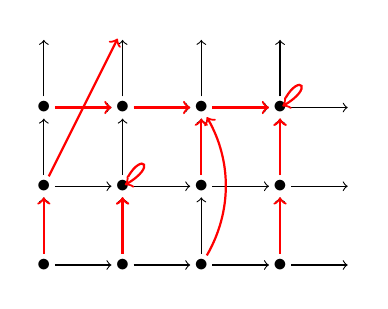
\begin{tikzpicture}[shorten <=4pt, shorten >=4pt]
	\foreach \i in {0,1,2,3} 
	{
		\foreach \j in {0,1,2}
		{
			\node (\i\j) at (\i,\j) {$\bullet$};
			\draw[->] (\i,\j) -- (\i+1,\j);
			\draw[->] (\i,\j) -- (\i,\j+1);
		};
	};
	\begin{scope}[red, thick]
		\draw[->] (0,0) -- (0,1);
		\draw[->] (0,1) -- (1,3);
		\draw[->] (0,2) -- (1,2);
		\draw[->] (1,0) -- (1,1);
		\draw[->] (1,1) edge[in=30, out=60, loop] (1,1);
		\draw[->] (1,2) -- (2,2);
		\draw[->] (2,0) to[bend right] (2,2);
		\draw[->] (2,1) -- (2,2);
		\draw[->] (2,2) -- (3,2);
		\draw[->] (3,0) -- (3,1);
		\draw[->] (3,1) -- (3,2);
		\draw[->] (3,2) edge[in=30, out=60, loop] (3,2);
	\end{scope}
\end{tikzpicture}
\]

For any category $\cat{C}$, the set of trajectories in $\cat{C}$ is in bijection with the set of cofunctors
\[
\cat{C}\cof\cat{N}
\]
where $\cat{N}$ is the monoid of natural numbers.
\end{example}

\begin{exercise}[Continuous trajectories]
If we say that a continuous trajectory in $\cat{C}$ is a cofunctor $\cat{C}\to\cat{R}$, where $\cat{R}$ is the monoid of real numbers under addition, considered as a category with one object. 

Describe continuous trajectories in $\cat{C}$ using elementary terms, i.e.\ to someone who doesn't know what a cofunctor is and doesn't yet want to learn.
\end{exercise}

\begin{example}[Very well-behaved lenses]
Recall that for any set $S$, we have the ``state'' comonoid $(S\yon^S,\epsilon,\delta)$ from \cref{ex.state_comonad_1}. What are the comonoid morphisms between them?

**Finish**
\end{example}

\begin{proposition}[Niu]
The coproduct of comonoids agrees with the coproduct of categories. In particular, the initial comonoid is $0$.
\end{proposition}

\begin{exercise}
Check that the terminal comonoid is $\yon$.
\end{exercise}

\begin{proposition}[Niu]
The category $\smcat^\sharp$ has products.

If $c$ and $d$ are the carriers of comonoids $\com{C}$ and $\com{D}$, then the carrier of $\com{C}\times\com{D}$ has carrier given by the following limit
\[
\begin{tikzcd}[column sep=23pt]
	\yon\ar[d]&
	\fl{c}\fl{d}\ar[d]&
	(\fl{c}\tri\fl{d})(\fl{d}\tri\fl{c})\ar[d]&
	(\fl{c}\tri\fl{d}\tri\fl{c})(\fl{d}\tri\fl{c}\tri\fl{d})\ar[d]&
	\cdots\\
	\1&
	(\fl{c}\tri\1)(\fl{d}\tri\1)\ar[l]&
	(\fl{c}\tri\fl{d}\tri\1)(\fl{d}\tri\fl{c})\ar[l]&
	(\fl{c}\tri\fl{d}\tri\fl{c}\tri\1)(\fl{d}\tri\fl{c}\tri\fl{d}\tri\1)\ar[l]&
	\cdots\ar[l]
	\end{tikzcd}
\]
where $\fl{c}$ and $\fl{d}$ are the fleeces of $c$ and $d$.
\end{proposition}

\paragraph{Results about cofunctors}
We refer to morphisms between polynomial comonoids as cofunctors, again eliding the difference between comonoids in $\poly$ and categories.

\begin{proposition}
Let $\Cat{Comon}(\poly)_{\text{rep}}$ be the full subcategory of comonoids $(c,\epsilon,\delta)$ in $\poly$ for which the carrier $c=\yon^M$ is representable. Then there is an isomorphism of categories
\[
\Cat{Comon}(\poly)_{\text{rep}}\cong\Cat{Mon}\op
\]
where $\Cat{Mon}$ is the category of monoids.
\end{proposition}
\begin{proof}
**
\end{proof}


\begin{exercise}
$\Cat{Comon}(\poly)_{\text{lin}}$ be the full subcategory of comonoids $(c,\epsilon,\delta)$ in $\poly$ for which the carrier $c=M\yon$ is linear. Show that there is an isomorphism of categories
\[
\Cat{Comon}(\poly)_{\text{lin}}\cong\smset
\]
\end{exercise}

\paragraph{Databases}

Discrete opfibrations will be important in our story, so let's spend a bit of time on them. It turns out that discrete opfibrations on a category have a close relationship with databases. Let's start with a definition.


\begin{definition}[Discrete opfibration]
A functor $F\colon\cat{C}\to\cat{D}$ is called a \emph{discrete opfibration} if, for every object $c\in\cat{C}$, object $d'\in\cat{D}$, and morphism $g\colon F(c)\to d'$ there exists a unique object $c'\in\cat{C}$ and morphism $f\colon c\to c'$ such that $F(c')=d'$ and $F(f)=g$.
\[
\begin{tikzcd}
  c\ar[r, dashed, "f"]\ar[d, |->, "F"']&
  c'\ar[d, |->, "F"]\\
  F(c)\ar[r, "g"']&
  d'
\end{tikzcd}
\]
\end{definition}


\begin{proposition}\label{prop.dopf_copresheaf}
Given a functor $\cat{C}\to\smset$, its category of elements is a discrete opfibration over $\cat{C}$, and this is functorial. Moreover this functor is an equivalence of categories.
\end{proposition}


\begin{example}[Database]
\end{example}



\begin{proposition}\label{prop.cart_com_dopf}
The category of polynomial comonoids and cartesian maps is equivalent to the category of categories and discrete opfibrations
\[
\Cat{Comon}(\poly)_{\text{cart}}\cong \smcat_{\text{dopf}}.
\]
\end{proposition}
\begin{proof}
**
\end{proof}

\begin{example}
Let $S$ be a set and $\com{S}\coloneqq(S\yon^S,\epsilon,\delta)$ the state comonoid. Then by \cref{prop.dopf_copresheaf,prop.cart_com_dopf}, a comonoid $\com{C}$ equipped with a cartesian map $f\colon\com{C}\to\com{S}$ is the category of elements for a functor $\cat{S}\to\smset$. But $\cat{S}$ is terminal in $\smcat$, so every functor $F\colon \cat{S}\to\smset$ is constant on some set $X\in\smset$, and hence there is an isomorphism of categories $\cat{C}\cong X\times \cat{S}$.
\end{example}

\begin{proposition}\label{prop.com_vert_cat_boo}
The category of polynomial comonoids and vertical maps is equivalent to the opposite of the category of categories and bijective-on-objects functors,
\[
\Cat{Comon}(\poly)_{\text{vert}}\cong(\smcat_{\text{boo}})\op.
\]
\end{proposition}
\begin{proof}
**
\end{proof}

\begin{exercise}
Let $S$ be a set and consider the state comonoid $\com{S}\coloneqq(S\yon^S,\epsilon,\delta)$. Use \cref{prop.com_vert_cat_boo} to show that comonoids $\com{C}$ equipped with a vertical cofunctor $\com{S}\to\com{C}$ can be identified with categories with object-set $S$.
\end{exercise}

\begin{exercise}
Consider the categories $\cat{C}\coloneqq\fbox{$\bullet\tto\bullet$}$ and $\cat{D}\coloneqq\fbox{$\bullet\to\bullet$}$. There is a unique bijective-on-objects (boo) functor $F\colon\cat{C}\to\cat{D}$ and two boo functors $G_1,G_2\colon\cat{D}\to\cat{C}$.
\begin{enumerate}
	\item Write down the morphism $\ema{d}\to\ema{c}$ of emanation polynomials underlying $F$.
	\item Write down the morphism $\ema{c}\to\ema{d}$ of emanation polynomials underlying either $G_1$ or $G_2$.
\qedhere
\end{enumerate}
\end{exercise}

\begin{proposition}
Every morphism of polynomial comonoids $f\colon\com{C}\to\com{D}$ factors as a vertical morphism followed by a cartesian morphism
\[
\com{C}\To{\text{vert}}\com{C}'\To{\text{cart}}\com{D}.
\]
\end{proposition}
\begin{proof}
**
\end{proof}

We can now give a third equivalent formulation of cofunctors and comonoid morphisms.

\begin{proposition}
The following categories are equivalent:
\begin{enumerate}
	\item The category $\smcat^\sharp$ of categories and cofunctors,
	\item The category $\Cat{Comon}(\poly)$ of polynomial comonoids, and
	\item The category whose objects are categories, morphisms $\cat{C}\to\cat{D}$ are spans of functors $\cat{C}\From{B}\cat{C}'\To{F}\cat{D}$, where $B$ is bijective on objects and $F$ is a discrete op-fibration; and composition is the usual composition of spans (by pullback in $\smcat$).
\end{enumerate}
\end{proposition}
\begin{proof}
**
\end{proof}


%-------- Section --------%
\section{Cofree comonoids}

\begin{proposition}
Let $p$ be a polynomial and $\cofree{p}$ the cofree comonoid. Every morphism in $\cat{C}_p$ is epic.
\end{proposition}

%-------- Section --------%
\section{Bimodules}

Bimodules with carrier $\yon$

\begin{theorem}
For a category $\cat{C}$ (comonoid $\com{C}$), the following are equivalent:
\begin{enumerate}
	\item functors $\cat{C}\to\smset$
	\item discrete opfibrations over $\cat{C}$
	\item cartesian cofunctors to $\com{C}$
	\item linear left $\com{C}$-modules
	\item constant left $\com{C}$-modules
	\item representable right $\com{C}$-modules
\end{enumerate}
\end{theorem}

\end{document}